
% JOD appendicies
\appendix

   %\section{Appendixes}
    \newpage
    \section{JOD Distribution}
   
   
   JOD is distributed\index{installation!distribution} as a \emph{J addon}.  
   You can install JOD using \texttt{pacman} the  
   \href{https://code.jsoftware.com/wiki/Pacman}{\emph{J package manager}} \cite{jwiki:jal}.
   
   
   The JOD distribution is broken into three \texttt{pacman} packages:
   \begin{enumerate}
	\item  \href{https://www.jsoftware.com/jwiki/Addons/general/jod}{\texttt{jod}} 
	\cite{baker:jod}:  This is the only package that must be installed to run JOD.  
	It contains  JOD system code and supporting files.
	\item  \href{https://www.jsoftware.com/jwiki/Addons/general/jodsource}{\texttt{jodsource}}
	 \cite{baker:jodsource}: This addon consists of three 
	   JOD dictionary dumps and a setup script.  JOD dictionary dumps\index{dictionary!source!\texttt{jodsource}}
	  are J script files that can rebuild  JOD dictionaries.  Dump files are the best way to
	  distribute dictionary code since they are independent of J binary representations. 
	  The \texttt{jodsource}\index{source code} addon contains.
  \begin{enumerate}
	  \item \texttt{joddev.ijs} --- development put dictionary\index{put dictionary}
	  \item \texttt{jod.ijs} --- main JOD source and test script dictionary
	  \item \texttt{utils.ijs}  --- common utilities dictionary
     \item \texttt{jodsourcesetup.ijs} --- J script that creates and loads the three
     JOD development dictionaries.
  \end{enumerate}
  \item \href{https://www.jsoftware.com/jwiki/Addons/general/joddocument}{\texttt{joddocument}} \cite{baker:joddocument}: this package contains 
  JOD PDF documents. Installing this
  package places these documents on local drives 
  for \hyperlink{il:jodhelp}{\texttt{jodhelp}}, see page~\pageref{ss:jodhelp}.  
\end{enumerate}

The \emph{packages} listed above are built from source scripts that are found in several GitHub\index{GitHub} repositories. To access raw  
JOD code see:  

\begin{enumerate}
\item The official \href{https://www.jsoftware.com}{\texttt{jsoftware.com}} repositories are:
\begin{enumerate}
\item \url{https://github.com/jsoftware/general_jod}
\item \url{https://github.com/jsoftware/general_joddocument}
\item \url{https://github.com/jsoftware/general_jodsource}
\end{enumerate}

\item My development repositories are:
\begin{enumerate}
\item \url{https://github.com/bakerjd99/jod}
\item \url{https://github.com/bakerjd99/joddumps}
\end{enumerate}

\item \LaTeX\ source for this document is at:
\begin{enumerate}
\item \url{https://github.com/bakerjd99/joddoc}
\end{enumerate}

\end{enumerate}

 \newpage
    \section{Building JOD}
    
    JOD is an open-source system. Anyone is free to examine and modify JOD source code. 
    All JOD source is stored in JOD development dictionaries. Installing the
    \href{https://www.jsoftware.com/jwiki/Addons/general/jodsource}{\texttt{jodsource}}\index{dictionary!source!\texttt{jodsource}}
    addon makes this code available. 
    
    JOD dictionaries also contain utilities for building\index{building!JOD distribution} and distributing JOD. 
    
\begin{lstlisting}[frame=single,framerule=0pt,basicstyle=\ttfamily\footnotesize]    
NB. open JOD development dictionaries
od ;:'joddev jod utils' [ 3 od ''

NB. before building create required directories
NB. directory creation is a one time step
'test' getrx 'setbuilddirs'
1 setbuilddirs_test_ 0

NB. build JOD
rm 'buildjoddistribution'
\end{lstlisting}   
    
   \texttt{buildjoddistribution} extracts JOD source code from development dictionaries and generates the compressed or 
    \href{https://en.wikipedia.org/wiki/Minification_(programming)}{\emph{minimized}} scripts 
    used by the JOD addon.
    
\begin{lstlisting}[frame=single,framerule=0pt,basicstyle=\ttfamily\footnotesize]
NB.*buildjoddistribution s-- full JOD distribution build.

cocurrent 'base'
cocurrent jodtestlocale 'AAAbuildjoddistribution'

NB. record open dictionaries and open JOD dictionaries
od ;:'joddev jod utils' [ 3 od'' [ ooo=: }. did 0

NB. get JOD build utilities and version tracking nouns
tmploc get }. grp 'buildjod'

NB. set distribution directories
jddir=: 'JODDOCDIR JODSTAGEDIR JODGITDIR JODSOURCESTAGEDIR JODSTAGEPDFDIR JODSTAGEDOCDIR'
jddir=: jddir , ' JODGITDOCDIR JODADDONDIR JODSCRIPTDIR JODEXTSDIR' 
(jddir)=: setbuilddirs 0

NB. generate distribution scripts
updatejodmanifest 0
JODVMD buildjodcompressed JODSTAGEDIR;JODGITDIR;JODADDONDIR;JODSCRIPTDIR
JODTOOLSVMD buildjodtoolscompressed JODSTAGEDIR;JODEXTSDIR;JODSCRIPTDIR
JODVMD updatejoddistribution JODSTAGEDIR;JODGITDIR;JODDOCDIR
JODVMD updatejodsourcedumps JODSOURCESTAGEDIR
JODVMD releasejod JODSTAGEDIR;JODSTAGEPDFDIR;JODSTAGEDOCDIR;JODGITDOCDIR

NB. destroy build locale
cocurrent 'base'
coerase <testlocale_ijod_
\end{lstlisting}

   \newpage
    \section{Testing JOD}\index{testing!running test scripts}

 Software is either \emph{tested} or \emph{trash}! There are no other
options! JOD aspires to be more than trash. So, it shouldn't surprise
anyone to learn that JOD development dictionaries contain many test
scripts. Test scripts are organized into \emph{suites}. Suites are
collections of test scripts.

\begin{lstlisting}[frame=single,framerule=0pt,basicstyle=\ttfamily\footnotesize]    
    NB. open JOD development dictionaries to use test scripts.
    od ;:'joddev jod utils' [ 3 od ''

    NB. make jodtester script - used by most test scripts
    mls 'jodtester'

    NB. list JOD test suites
    80 list }. 3 dnl 'jod'
jodbasictests     jodcrushtests     joddualsystests   jodextensiontests 
jodlargetests     jodmanwintests    jodpjmtest        jodpreparetests   
jodpurgetests     jodsmoketests     jodstresstests  
\end{lstlisting} 

\noindent Because test scripts are often more revealing and informative than
standard documentation, I have posted them on GitHub at

\medskip
\small \url{https://github.com/bakerjd99/jod/tree/master/jodunit}. \normalsize 
\medskip

\noindent The majority
of the scripts can be run with JOD's \hyperlink{il:rtt}{\texttt{rtt}} verb, see page~\pageref{ss:rtt}.

\begin{lstlisting}[frame=single,framerule=0pt,basicstyle=\ttfamily\footnotesize]    
    NB. run silently - only explict output shown - expected result is 1
    1 rtt 'bnlSmoke02'

    NB. show all input and output
    rtt  'bnlSmoke02'
\end{lstlisting} 

\noindent The following test script is typical of JOD tests. Run with {\texttt{rtt}}.

\begin{lstlisting}[frame=single,framerule=0pt,basicstyle=\ttfamily\footnotesize] 
NB.*bnlSmoke02 t-- (bnl) test hash failure detection.

cocurrent 'base'
require 'jodtester'

cocurrent jodtestlocale 'AAAbnlSmoke02'

testenvironment 'good';'JOD'
NB. -{TEST START}-

NB. is folder configured
iscf '~JODTEST'

NB. set test dictionary
er settdict tdict=: 'testjod00'

NB. read and write bytes
read=: 1!:1&(]`<@.(32&>@(3!:0)))
write=: 1!:2 ]`<@.(32&>@(3!:0))

NB. close any open and open test dictionary
er od tdict [ 3 od ''

NB. erase any current test dictionary backups
DL=: {: {.DPATH__ST__JODobj
0 0$ferase 1 dir BAK__DL,'*.*'

NB. no backup error expected
ner 14 bnl '.'

NB. insert random arrays  between backups to insure
NB. hashes in the njhashes.txt sidecar files differ
hashhack=: ?5 5 5$1000000
hashmsg=: 'first backup'
er tmploc put 'hashhack'
er tmploc put 'hashmsg'
er packd tdict

hashhack=: ?5 5 5$1000000
hashmsg=: 'second backup'
er tmploc put 'hashhack'
er tmploc put 'hashmsg'
er packd tdict

NB. all hashes should pass
er showpass hashes=: 17 bnl '.'
*./ ; 1 1 }. rv_ajod_ hashes

NB. copy and rename older backup word files over
NB. newer backups - this will introduce a hash failure
jwords=: dirtree BAK__DL,'*jwords.ijf'
jwords=: (\: 1 {"1 jwords){jwords
(read ;0{{:jwords) write ;0{{.jwords
er showpass hckhashes=: 17 bnl '.'

NB. some hashes fail - 0s in 17 bnl '.'
0 e. ; 1 1 }. rv_ajod_ hckhashes

NB. -{TEST SUCCESSFUL}-
ereopen 0

cocurrent 'base'
coerase <testlocale_ijod_
\end{lstlisting}   

    
     
   \newpage
   \section{JOD Classes}\label{ap:classes}
   
   \begin{figure}[htbp]
  \centering
  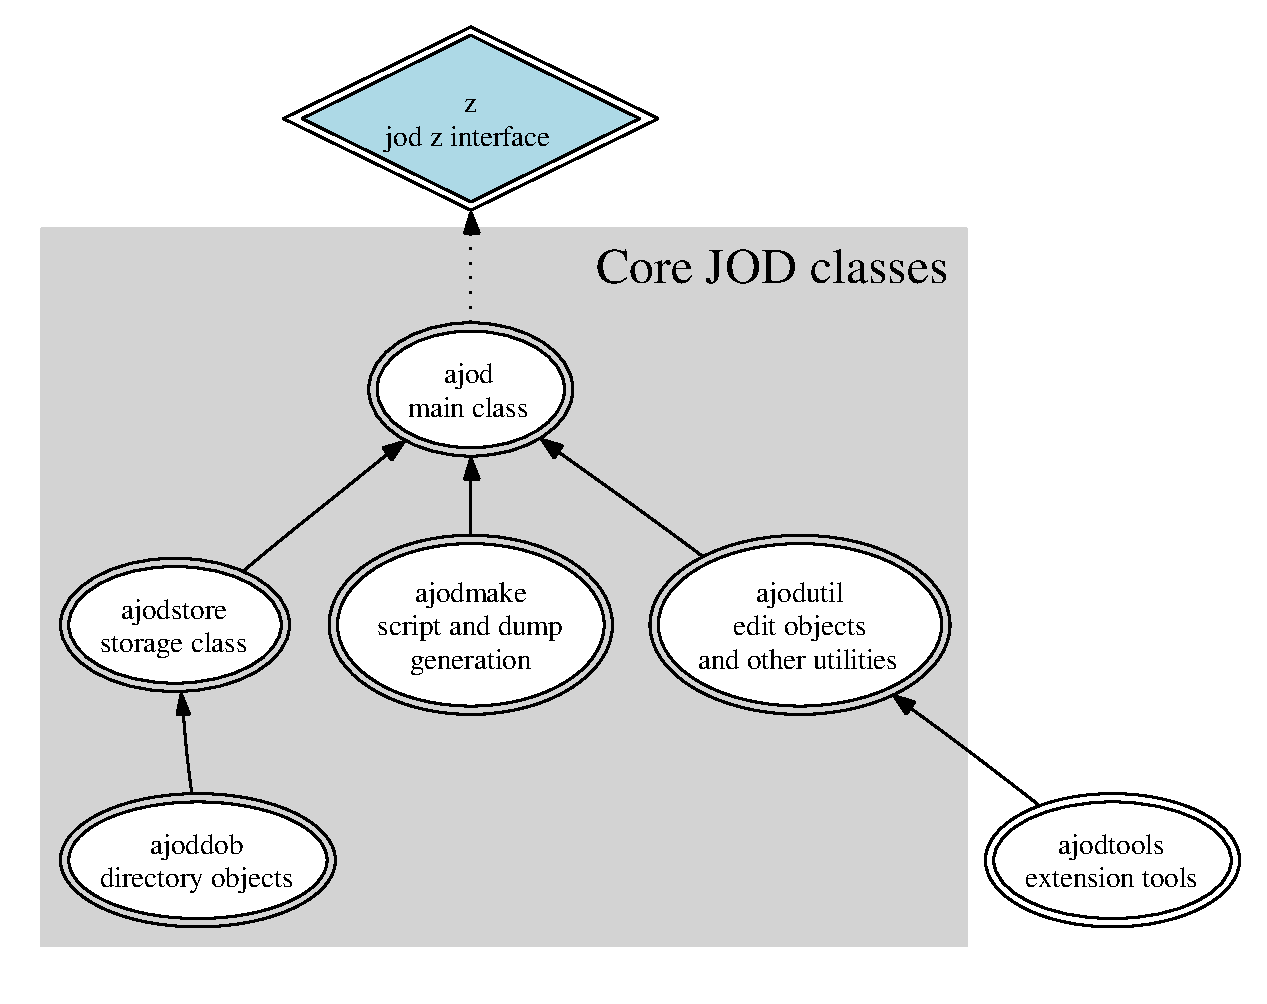
\includegraphics[width=0.84\textwidth]{joddot}
  \caption[JOD Classes]{This diagram\index{z interface}\index{ijod interface} shows how 
    JOD classes\index{classes} are related. JOD classes are loaded into 
    J addon \textbf{\texttt{a}} locales. The arrows\index{locale!classes} indicate how J names are resolved.
    The \emph{blue diamond} locales \texttt{ijod} and \texttt{z} are on the \texttt{base} locale's 
    path: \texttt{copath 'base'}. \emph{Diagram Generated by} \texttt{Graphviz} \cite{jwiki:graphviz}.    
    }
   \label{eps:joddot}
   \end{figure}
   
   \newpage
   \section{Reference Path}\label{ap:refpath}
   
   JOD groups and suites, (see \hyperlink{il:grp}{\texttt{grp}} on page~\pageref{ss:grp}), are defined with respect to a particular path.  This path is called the \emph{reference path}.  The reference path\index{reference path} is stored when the first put dictionary group or 
suite is defined.   Group and suite generation with \hyperlink{il:make}{\texttt{make}}, \hyperlink{il:mls}{\texttt{mls}} and  \hyperlink{il:lg}{\texttt{lg}}, (see pages~\pageref{ss:make}, \pageref{ss:mls}, \pageref{ss:lg}), check the current path against the reference path.  If the paths do not match an error is returned.

Reference paths display current dictionary names but the path is 
stored as a unique list of extended dictionary 
identification numbers: \texttt{DIDNUM}s.  On Windows and Linux 
systems the \texttt{DIDNUM}\index{DIDNUM} is based 
on \texttt{GUID}s.  \texttt{DIDNUM}s insure reference paths are unique.


A reference path can only be reset by clearing the put dictionary\index{put dictionary}
 path, opening desired dictionaries and recreating a group or suite: see \hyperlink{il:dpset}{\texttt{dpset}} on page~\pageref{ss:dpset}.

\begin{lstlisting}[frame=single,framerule=0pt,basicstyle=\ttfamily\footnotesize]
    NB. open first five dictionaries 
    od 5 {. }. od ''
+-+--------------------------+------+---+-----+--------+---+
|1|opened (rw/rw/ro/rw/rw) ->|budget|cbh|flick|flickdev|gps|
+-+--------------------------+------+---+-----+--------+---+

    NB. display dictionary information - reference paths in last column
    did ~ 0
+-+----------------------------------------------------------------------+
|1|+--------+--+-----+-----+-------+-------+------+---------------------+|
| ||        |--|Words|Tests|Groups*|Suites*|Macros|*Path                ||
| |+--------+--+-----+-----+-------+-------+------+---------------------+|
| ||budget  |rw|14   |0    |2      |0      |0     |/budget              ||
| |+--------+--+-----+-----+-------+-------+------+---------------------+|
| ||cbh     |rw|145  |0    |6      |0      |6     |/cbh/utils           ||
| |+--------+--+-----+-----+-------+-------+------+---------------------+|
| ||flick   |ro|296  |3    |9      |0      |9     |/flick/utils         ||
| |+--------+--+-----+-----+-------+-------+------+---------------------+|
| ||flickdev|rw|96   |2    |2      |0      |2     |/flickdev/flick/utils||
| |+--------+--+-----+-----+-------+-------+------+---------------------+|
| ||gps     |rw|11   |0    |0      |0      |0     |/gps/utils           ||
| |+--------+--+-----+-----+-------+-------+------+---------------------+|
+-+----------------------------------------------------------------------+
\end{lstlisting}
   
   \newpage
   \section{JOD Argument Codes}\label{ap:objqualcodes}

The left, and some right, arguments of JOD verbs are specified with \emph{object}, \emph{qualifier} and \emph{option} codes. Object codes\index{codes!argument} are typically the first argument code while options and qualifiers usually occupy the second and third positions. Options and qualifiers are sometimes negative. Negative values modify codes: see tables~\ref{tab:objcodes}, \ref{tab:objneg} and
\ref{tab:qualcodes} on pages~\pageref{tab:objcodes},  \pageref{tab:objneg} and \pageref{tab:qualcodes}.

\begin{table}[htbp]
  \centering
   \scriptsize
   \begin{tabular}{|l|l|l|p{4.0in}|} \hline
   \multicolumn{4}{|c|}{\textbf{\normalsize Object Codes\T\B}} \\ \hline
   \multicolumn{1}{|c|}{\textbf{\normalsize Noun\T}} & 
   \multicolumn{1}{|c|}{\textbf{\normalsize Code}} & 
   \multicolumn{1}{|c|}{\textbf{\normalsize Use}} & 
   \multicolumn{1}{|c|}{\textbf{\normalsize Example\B}} \\ \hline
   \texttt{WORD\T\B} & 0 & word code & \begin{minipage}{3.9in}
\begin{tabular}{l}
\verb|0 dnl ''  | \textcolor{CodeComment}{\ttfamily\textsl{NB. list all words on path}} \\
\end{tabular} 
\end{minipage} \\ \hline
 \texttt{TEST\T\B} & 1 & test case code & \begin{minipage}{3.9in}
\begin{tabular}{l}
\verb|1 put 'test';'test code..'  | \textcolor{CodeComment}{\ttfamily\textsl{NB. store test}} \\
\end{tabular} 
\end{minipage} \\ \hline
 \texttt{GROUP\T\B} & 2 & group code & \begin{minipage}{3.9in}
\begin{tabular}{l}
\verb|2 put 'name';'group header ...'  | \textcolor{CodeComment}{\ttfamily\textsl{NB. store group header}} \\
\end{tabular} 
\end{minipage} \\ \hline
 \texttt{SUITE\T\B} & 3 & suite code & \begin{minipage}{3.9in}
\begin{tabular}{l}
\verb|3 grp 'suite'  | \textcolor{CodeComment}{\ttfamily\textsl{NB. get suite members, list of test names}} \\
\end{tabular} 
\end{minipage} \\ \hline
 \texttt{MACRO\T\B} & 4 & macro code & \begin{minipage}{3.9in}
\begin{tabular}{l}
\verb|4 disp 'test'  | \textcolor{CodeComment}{\ttfamily\textsl{NB. display macro}} \\
\end{tabular} 
\end{minipage} \\ \hline
 \texttt{DICTIONARY\T\B} & 5 & dictionary code & \begin{minipage}{3.9in}
\begin{tabular}{l}
\verb|5 get ''  | \textcolor{CodeComment}{\ttfamily\textsl{NB. get dictionary documentation}} \\
\end{tabular} 
\end{minipage} \\ \hline
    \end{tabular}
   \caption{JOD Object Codes}
  \label{tab:objcodes}
\end{table}

The meaning of negative option and qualifier codes depends on the word.  For 
\hyperlink{il:dnl}{\texttt{dnl}} a negative option requests a \emph{path order list.}\index{path order list}
For \hyperlink{il:get}{\texttt{get}} and \hyperlink{il:put}{\texttt{put}} a negative
option code gets and puts timestamp arrays.

\begin{table}[htbp]
  \centering
   \scriptsize
\begin{tabular}{|l|l|p{4.7in}|} \hline
   \multicolumn{3}{|c|}{\textbf{\normalsize Negative Codes\T\B}} \\ \hline
   \multicolumn{1}{|c|}{\textbf{\normalsize Code\T}} & 
   \multicolumn{1}{|c|}{\textbf{\normalsize Use}} & 
   \multicolumn{1}{|c|}{\textbf{\normalsize Example\B}} \\ \hline
   \verb|_1|\T\B & path order list & \begin{minipage}{3.9in}
\begin{tabular}{l}
\verb|0 _1 dnl ''  | \textcolor{CodeComment}{\ttfamily\textsl{NB. path order list of words}} \\
\end{tabular} 
\end{minipage} \\ \hline
\verb|_2|\T\B & path order list & \begin{minipage}{3.9in}
\begin{tabular}{l}
\verb|1 _2 dnl 'boo'  | \textcolor{CodeComment}{\ttfamily\textsl{NB. path order list of test names containing boo}} \\
\end{tabular} 
\end{minipage} \\ \hline
\verb|_14|\T\B & names and timestamps & \begin{minipage}{3.9in}
\begin{tabular}{l}
\verb|1 _14 get }. revo''  | \textcolor{CodeComment}{\ttfamily\textsl{NB. names and timestamps array}} \\
\end{tabular} 
\end{minipage} \\ \hline
\verb|_14|\T\B & names and timestamps & \begin{minipage}{3.9in}
\begin{tabular}{l}
\verb|4 _14 put tsarray  | \textcolor{CodeComment}{\ttfamily\textsl{NB. update macro timestamps}} \\
\end{tabular} 
\end{minipage} \\ \hline
\end{tabular}
   \caption{JOD Negative Codes}
   \label{tab:objneg}
\end{table}

\newpage

\begin{table}[htbp]
  \centering
   \scriptsize
   \begin{tabular}{|l|l|l|p{4.0in}|} \hline
   \multicolumn{4}{|c|}{\textbf{\normalsize Qualifier Codes\T\B}} \\ \hline
   \multicolumn{1}{|c|}{\textbf{\normalsize Noun\T}} & 
   \multicolumn{1}{|c|}{\textbf{\normalsize Code}} & 
   \multicolumn{1}{|c|}{\textbf{\normalsize Use}} & 
   \multicolumn{1}{|c|}{\textbf{\normalsize Example\B}} \\ \hline
   \texttt{DEFAULT\T\B} & 7 & default action & \begin{minipage}{3.9in}
\begin{tabular}{l}
\verb|0 7 get 'this'  | \textcolor{CodeComment}{\ttfamily\textsl{NB. default behaviour}} \\
\end{tabular} 
\end{minipage} \\ \hline
 \texttt{EXPLAIN\T\B} & 8 & short explanation text & \begin{minipage}{3.9in}
\begin{tabular}{l}
\verb|0 8 put 'name';'explain name'  |  \\
\end{tabular} 
\end{minipage} \\ \hline
 \texttt{DOCUMENT\T\B} & 9 & documentation text & \begin{minipage}{3.9in}
\begin{tabular}{l}
\verb|2 9 put 'group';'very long group document ...'  |  \\
\end{tabular} 
\end{minipage} \\ \hline
 \texttt{NVTABLE\T\B} & 10 & name value table & \begin{minipage}{3.9in}
\begin{tabular}{l}
\verb|0 10 get }. dnl ''  | \textcolor{CodeComment}{\ttfamily\textsl{NB. return all words in table}} \\
\end{tabular} 
\end{minipage} \\ \hline

 \texttt{REFERENCE\T\B} & 11 & reference code & \begin{minipage}{3.9in}
\begin{tabular}{l}
\verb|11 del 'earthdist'  | \textcolor{CodeComment}{\ttfamily\textsl{NB. delete word references}} \\
\end{tabular} 
\end{minipage} \\ \hline

 \texttt{NAMECLASS\T\B} & 12 & J name class code & \begin{minipage}{3.9in}
\begin{tabular}{l}
\verb|0 12 get }. dnl ''| \textcolor{CodeComment}{\ttfamily\textsl{NB. fetch J name class codes}} \\
\end{tabular} 
\end{minipage} \\ \hline

 \texttt{CREATION\T\B} & 13 & creation date & \begin{minipage}{3.9in}
\begin{tabular}{l}
\verb|0 13 get }. dnl ''| \textcolor{CodeComment}{\ttfamily\textsl{NB. word creation dates}} \\
\end{tabular} 
\end{minipage} \\ \hline

 \texttt{LASTPUT\T\B} & 14 & last change date & \begin{minipage}{3.9in}
\begin{tabular}{l}
\verb|0 14 get }. dnl ''| \textcolor{CodeComment}{\ttfamily\textsl{NB. recent changes}} \\
\end{tabular} 
\end{minipage} \\ \hline

\texttt{HASH\T\B} & 17 & hash code & \begin{minipage}{3.9in}
\begin{tabular}{l}
\verb|17 bnl '.'| \textcolor{CodeComment}{\ttfamily\textsl{NB. check backup files against hashes}} \\
\end{tabular} 
\end{minipage} \\ \hline

 \texttt{BYTESIZE\T\B} & 15 & object byte size & \begin{minipage}{3.9in}
\begin{tabular}{l}
\verb|0 15 get }. dnl ''| \textcolor{CodeComment}{\ttfamily\textsl{NB. word byte sizes}} \\
\end{tabular} 
\end{minipage} \\ \hline

 \texttt{JSCRIPT\T\B} & 21 &  J script code\index{postprocessor} & \begin{minipage}{3.9in}
\begin{tabular}{l}
\verb|4 1 21 dnl 'POST_'  | \textcolor{CodeComment}{\ttfamily\textsl{NB. list postprocessors}} \\
\end{tabular} 
\end{minipage} \\ \hline
\texttt{LATEX\T\B} & 22 & \LaTeX\ text code  & \begin{minipage}{3.9in}
\begin{tabular}{l}
\verb|4 get }. 4 3 22 dnl 'TEX'  | \textcolor{CodeComment}{\ttfamily\textsl{NB. get LaTeX macros}} \\
\end{tabular} 
\end{minipage} \\ \hline
\texttt{HTML\T\B} & 23 & HTML text code & \begin{minipage}{3.9in}
\begin{tabular}{l}
\verb|4 put 'HTMLtxt';23;'<a>hello world</a>'  | \textcolor{CodeComment}{\ttfamily\textsl{NB. store html}} \\
\end{tabular} 
\end{minipage} \\ \hline
\texttt{XML\T\B} & 24 & XML text code & \begin{minipage}{3.9in}
\begin{tabular}{l}
\verb|4 put 'XMLtext24;'<p>baby step xml</p>'  |  \textcolor{CodeComment}{\ttfamily\textsl{NB. store xml}}\\
\end{tabular} 
\end{minipage} \\ \hline
\texttt{TEXT\T\B} & 25 & ASCII text code & \begin{minipage}{3.9in}
\begin{tabular}{l}
\verb|4 3 25 dnl 'EPS'  | \textcolor{CodeComment}{\ttfamily\textsl{NB. texts ending with EPS}} \\
\end{tabular} 
\end{minipage} \\ \hline
\texttt{BYTE\T\B} & 26 & BYTE characters & \begin{minipage}{3.9in}
\begin{tabular}{l}
\verb|4 put 'BYTEME';a.|  \\
\end{tabular} 
\end{minipage} \\ \hline

\texttt{MARKDOWN\T\B} & 27 & \href{https://daringfireball.net/projects/markdown/}{MARKDOWN} text code & \begin{minipage}{3.9in}
\begin{tabular}{l}
\verb|5 put 'Main **dictionary** document' |  \\
\end{tabular} 
\end{minipage} \\ \hline

\texttt{UTF8\T\B} & 28 & Unicode UTF8 text & \begin{minipage}{3.9in}
\begin{tabular}{l}
\verb|4 put 'UTF8text';UTF8_ajod_;(8 u: 4 u: 56788 4578,65+i.5)  |  \\
\end{tabular} 
\end{minipage} \\ \hline

\texttt{PYTHON\T\B} & 29 & Python script text & \begin{minipage}{3.9in}
\begin{tabular}{l}
\verb|4 put 'big_py';PYTHON_ajod_;'2 ** 1024'  |  \\
\end{tabular} 
\end{minipage} \\ \hline

\texttt{SQL\T\B} & 30 & SQL script text & \begin{minipage}{3.9in}
\begin{tabular}{l}
\verb|4 put 'yada_sql';SQL_ajod_;'select * from yada'  |  \\
\end{tabular} 
\end{minipage} \\ \hline

\texttt{JSON\T\B} & 31 & JSON text & \begin{minipage}{3.9in}
\begin{tabular}{l}
\verb|4 put 'fleece_json';JSON_ajod_;'{"json": "golden-fleece"}'  |  \\
\end{tabular} 
\end{minipage} \\ \hline

\texttt{IPYNB\T\B} & 32 & \href{https://jupyter.org/}{Jupyter} notebook & \begin{minipage}{3.9in}
\begin{tabular}{l}
\verb|4 put 'notebook_ipynb';IPYNB_ajod_;'... ipynb ...'  |  \\
\end{tabular} 
\end{minipage} \\ \hline

\texttt{LEAN\T\B} & 33 & \href{https://leanprover-community.github.io/}{LEAN} source code & \begin{minipage}{3.9in}
\begin{tabular}{l}
\verb|4 put 'theorem_lean';LEAN_ajod_;'... lean on me ...'  |  \\
\end{tabular} 
\end{minipage} \\ \hline

\texttt{ZIG\T\B} & 34 & \href{https://ziglang.org/}{ZIG} source code & \begin{minipage}{3.9in}
\begin{tabular}{l}
\verb|4 put 'code_zig';ZIG_ajod_;'... ziggy code stuff ...'  |  \\
\end{tabular} 
\end{minipage} \\ \hline


%\texttt{PYTHON\T\B} & 29 & Python script text & \begin{minipage}{3.9in}
%\begin{tabular}{l}
%\verb|4 put 'PYTHONTEXT';PYTHON_ajod_;'2 ** 1024'  |  \\
%\end{tabular} 
%\end{minipage} \\ \hline
    \end{tabular}
   \caption{JOD Qualifier Codes}
  \label{tab:qualcodes}
\end{table}

\textbf{Note:} suffixes like \texttt{notebook\_ipynb} are not required. I use them to make it easier to see what type of code is stored in a JOD macro.

 
   \newpage
   \section{\texttt{jodparms.ijs}}\label{ap:jodparms}
   
\verb|jodparms.ijs| is read when the master file\index{master file} \verb|jmaster.ijf| is created
and is used to set dictionary parameters.

Dictionary parameters are distributed to dictionary files and runtime
objects. New parameters can be added by editing \verb|jodparms.ijs|
and recreating the master file.
The last few lines of the following example show how to add
\texttt{COPYRIGHT} and \texttt{MYPARAMETER}. 

When a parameter is added its value will appear in the directory
objects of all dictionaries but will only be \hyperlink{il:dpset}{\texttt{dpset}}'able in new dictionaries.

\begin{quotation}
	To change default master dictionary parameters:
	\begin{enumerate}
	  \item Exit J
		\item Delete the files
	  \begin{description}
		  \item \verb|~addons/general/jod/jmaster.ijf|
		  \item \verb|~addons/general/jod/jod.ijn|
  	\end{description}
		\item Edit 
  	\begin{description}
	 	  \item \verb|~addons/general/jod/jodparms.ijs|
  	\end{description}
		\item Restart J and reload JOD with 
		\begin{description}
	   	\item \verb|load 'general/jod'|
		\end{description}
	 \end{enumerate}
\end{quotation}

%\vspace{0.5cm}	

\begin{lstlisting}[frame=single,framerule=0pt,basicstyle=\ttfamily\footnotesize]
NB.*jodparms s-- default dictionary parameters.
NB.
NB. This file is used to set  the  default  dictionary parameters
NB. table  in the master file. When  a  new dictionary is created
NB. the  parameters  in the  master file are used to specify  the
NB. parameters for a particular dictionary. The  verb (dpset) can
NB. be   used  to   modify  parameter  settings   in   individual
NB. dictionaries.  Master  file parameters can only be changed by
NB. editing this file and recreating the master file.
NB.
NB. The master file can be recreated with the call:
NB.
NB. createmast_ajod_ JMASTER_ajod_
NB.
NB. WARNING: all the  parameters currently listed are required by
NB. the JOD system. If you remove any of them JOD will crash. You
NB. can  safely add additional parameters but  you  cannot safely
NB. remove current parameters.

MASTERPARMS=: 0 : 0

NB. The format of this parameter file is:
NB.     jname ; (type) description ; value
NB. 
NB.     jname is a valid J name
NB.     (type) description documents the parameter - type is required
NB.        only (+integer) is currently executed other types will
NB.        be passed as character lists (see dptable).
NB.     value is an executable J expression that produces a value

ASCII85    ; (+integer) when 1 use ascii85 in dumps (0 or 1) ; 1  
COPYFACTOR ; (+integer) components copied in one loop pass  (1<y<240) ; 100
DOCUMENTDICT ; (+integer) when 1 dictionary document is put (0 or 1)  ; 1
DOCUMENTWIDTH ; (+integer) width of justified document text  (20<y<255) ; 61
DUMPFACTOR ; (+integer) objects dumped in one loop pass (1<y<240)     ; 50
GETFACTOR  ; (+integer) words retrieved in one loop pass (10<y<2048)  ; 250
PUTFACTOR  ; (+integer) words stored in one loop pass  (10<y<2048)    ; 100
RETAINAGE  ; (+integer) when 1 timestamps are saved in dumps (0 or 1) ; 1
HASHDUMP   ; (+integer) when 1 a hash is prefixed to dumps (0 or 1)   ; 1

NB. ROOTFOLDER is empty by default. If it is set to a (jpath) J configured 
NB. folder ROOTFOLDER overrides default locations for (mls) generated scripts 
ROOTFOLDER ; (character) redirects (mls) scripts to J folder ; 

NB. typical nonempty setting
NB. ROOTFOLDER ; (character) redirects (mls) scripts to J folder ; ~user/jodroot 

NB. Any added parameters are stored in the master file when
NB. created and distributed to JOD directory objects.  

NB. WARNING: when defining J expressions be careful about the ; character 
NB. the JOD code (dptable) that parses this string is rudimentary.

NB. COPYRIGHT ; (character) ; All rights reserved
NB. MYPARAMETER ; (+integer) the answer ; 42
)
\end{lstlisting}


   \newpage
   \section{\texttt{jodprofile.ijs}}\label{ap:jodprofile}
   
\verb|jodprofile.ijs| is an optional user profile script; it runs after
JOD loads and can be used to customize\index{configuration!\texttt{jodprofile.ijs}} your working environment.  The following is an example
profile script. 

%\lstset{numbers=left, numberstyle=\tiny, stepnumber=2, numbersep=5pt}

\begin{lstlisting}[frame=single,framerule=0pt,basicstyle=\ttfamily\footnotesize]
NB.*jodprofile s-- JOD dictionary profile.
NB.
NB. An example JOD profile script. Save this script in
NB.
NB. ~addons/general/jod/
NB.
NB. with the name jodprofile.ijs
NB.
NB. This script  is  executed  after all dictionary  objects have
NB. been created. It  can  be used  to  set up  your default  JOD
NB. working environment.

NB. set white space preservation on
9!:41 [ 1

NB. minimum print precision to show yyyymmdd dates (see jodage)
9!:11 [ 8

NB. set jqt windows console size - automatic for linux/mac/ios
Cwh_j_=: 160 24

NB. do not reset if you are running more than one JOD instance
NB. multiple JOD instances are permitted but not recommended
dpset 'RESETME'

NB. JOD interface locale - (ijod) is a good place for ad hoc JOD addons
coclass 'ijod'

NB. used by some macros: WHEREAMI=: ;0 { ;:'home work test'
WHEREAMI=: 'home'

NB. (ijod) error/ message text
ERRIJOD00=: 'current group name (jodg_ijod_) not set'
ERRIJOD01=: 'current suite name (jods_ijod_) not set'
ERRIJOD02=: 'invalid (x) search string'
OKIJOD00=:  'no matches'
OKIJOD01=:  'no objects'

NB. add delete objects from current group or current suite
ag=: {{if. wex_ajod_ <'jodg' do. jodg addgrp y else. jderr_ajod_ ERRIJOD00 end.}}
as=: {{if. wex_ajod_ <'jods' do. (jods;3) addgrp y else. jderr_ajod_ ERRIJOD01 end.}}
dg=: {{if. wex_ajod_ <'jodg' do. jodg delgrp y else. jderr_ajod_ ERRIJOD00 end.}}
ds=: {{if. wex_ajod_ <'jods' do. (jods;3) delgrp y else. jderr_ajod_ ERRIJOD01 end.}}
   
NB. referenced words not in current group
nx=: 3 : 0
if. -.wex_ajod_ <'jodg' do. jderr_ajod_ ERRIJOD00 return. end.
if. badrc_ajod_ gn=. grp jodg do. gn return. end.
(allrefs  }. gn) -. gn
)
   
NB. words in current group using a word
ug=: 3 : 0
if. -.wex_ajod_ <'jodg' do. jderr_ajod_ ERRIJOD00 return. end.
if. badrc_ajod_ gn=. grp jodg do. gn return. end.
y usedby }. gn
)
   
NB. generate current group and save load script
sg=: {{if. wex_ajod_ <'jodg' do. mls jodg else. jderr_ajod_ ERRIJOD01 end.}}

NB. open entire (y) path
oep=: 6&od

NB. top (put dictionary) words, groups, suites in revision order
tw=: revo
tg=: 2&revo
ts=: 3&revo

NB. run tautology as plaintest - does not stop on nonzero results
rt=: 2&rtt

NB. run tautology silently - will show explict smoutput
rq=:1&rtt

NB. run macro silently - will show explict smoutput
rs=: 1&rm

NB. short help for groups/suites
hg=: [: hlpnl [: }. grp
hs=: 1 hlpnl [: }. 3 grp ]

NB. short help on put objects in revised order from code:
NB.     hr 4  NB. macro
NB.     hr 2  NB. groups
NB.  10 hr 0  NB. last ten words
hr=: 3 : 0
if. badrc_ajod_ w=. y revo '' do. w return. end.
y hlpnl }. w
:
if. badrc_ajod_ w=. y revo '' do. w return. end.
y hlpnl x {. }. w
)

NB. remove trailing blank rows
rebtbrow=: ] #~ [: -. [: *./"1 [: *./\. ' '&=

NB. appends trailing line feed character if necessary
tlf=:] , ((10{a.)"_ = {:) }. (10{a.)"_

NB. show long documents
NB.      hld 0     NB. words
NB.      hld 2     NB. groups
NB.  0 1 0 hld 0   NB. documented nouns
NB. 'NIMP:' hld 0  NB. word docs with string 'NIMP:'
NB.  (] ,: #@hld"0) i. 5 NB. count docs on path
hld=: ''&$: :(4 : 0)
if. badcl_ajod_ x do. jderr_ajod_ ERRIJOD02 return. end.
if. badrc_ajod_ w=. y dnl '' do. w return. end.
if. 0=#&> w=. }. w do. ok_ajod_ OKIJOD01 return. end.
if. badrc_ajod_ d=. (({.y),9) get w do. d return. end.
d=. d #~ 0 < #&> 1 {"1 d=. >1{d
if. 0<#x do. d=. d #~ +./@(x&E.)&> 1 {"1 d end.
(0 {"1 d) ,. rebtbrow@(];._2)@tlf@(-.&CR)&.> 1 {"1 d
)

NB. search short help for string and list matching words
NB.     hss 'see long'   NB. search word short text 
NB.  2  hss 'see long'   NB. search group short text
NB.  4  hss 'post'       NB. search macro short text 
hss=: 0&$: :(4 : 0)
if. badrc_ajod_ w=. x dnl ''   do. w return. end.
d=. x hlpnl }. w
if. 0=#w=. 1 >@{ d             do. ok_ajod_ OKIJOD00 return. end.
if. 0=#s=. I. (,:y) +./"1@E. w do. ok_ajod_ OKIJOD00 return. end.
s&{ &.> d
)

NB. single line explanation 
NB.    slex 'word'         NB. word
NB.  4 slex 'jodregister'  NB. macro
NB.  1 slex 'thistest'     NB. test
slex=: 0&$: :(4 : 0)
if. badcl_ajod_ sl=. x disp y do. sl return. end.
(x,8) put y;firstcomment__JODtools sl
)

NB. regenerate put dictionary word cross references
reref=: 3 : 0
if. badrc_ajod_ r=. revo '' do. r return. end.
(r,.s) #~ -.;0{"1 s=.0 globs&> r=.}.r
)

NB. handy cl doc helpers
docscr=: {{ctl_ajod_ (61;0;0;'NB.') docct2__UT__JODobj ];._1 LF,y-.CR}}
doctxt=: {{ctl_ajod_ (61;0;0;'') docct2__UT__JODobj ];._1 LF,y-.CR}}

NB. display noun on screen and return noun value
showpass=:] [ 1!:2&2

NB. portable box drawing characters
portchars=:[: 9!:7 '+++++++++|-'"_ [ ]

NB. windows lucida console box drawing characters
winlcchars=:[: 9!:7 (a.{~16+i.11)"_ [ ]

NB. edit command 
DOCUMENTCOMMAND=: 'showpass pr ''{~N~}'''

NB. read & write files
read=:1!:1&(]`<@.(32&>@(3!:0)))
write=:1!:2 ]`<@.(32&>@(3!:0))
readnoun=:3!:2@(1!:1&(]`<@.(32&>@(3!:0))))
writenoun=:([: 3!:1 [) (1!:2 ]`<@.(32&>@(3!:0))) ]

NB. fetch edit text/macros and associate code
tt=:] ; gt
mt=:] ; 25"_ ; gt   NB. *.txt
mj=:] ; 21"_ ; gt   NB. *.ijs
md=:] ; 27"_ ; gt   NB. *.markdown
mq=:] ; 30"_ ; gt   NB. *.sql
mx=:] ; 22"_ ; gt   NB. *.tex

NB. ~user/temp object text - default j script
os=: 'ijs'&$: : ([: jpath '~user/temp/' , (' ' -.~ ]) , '.' , ' ' -.~ [)
 
NB. read text from j user temp directory
jt=:[: read os
 
NB.  load j script from j user temp
jl=: (0!:0)@jt

NB. load j script from configured j path
jp=: [: 0!:0 [: < jpath

NB. load and show j script from configured path
jps=: [: 0!:001 [: < jpath

NB. number of objects - used by various (utils) macros (sizeput, ageput, ...) if present
NOBS=: 10

NB. show (1) or suppress (0) dyadic (smoutput)
SHOWSMO=: 1

NB. create temporary named and labeled jod test locales for j 9.6 and beyond
NB. NOTE: WARNING: (jodtestlocale) is used in most JOD test scripts.
(3 : 0) ''
if. 9.6 <: jvn_ajod_'' do.
jodtestlocale=: {{'ijod' jodtestlocale y 
: 
((;:x),copath y) copath y [ _1 cocreate <y [ coerase <y=. y -. ' '
('tmploc_',y,'_')=: y [ testlocale_ijod_=:y}}
else.
jodtestlocale=: {{'ijod' jodtestlocale y 
: 
((;:x),copath y) copath y [ cocreate <y [ coerase <y=. y -. ' '
('tmploc_',y,'_')=: y [ testlocale_ijod_=: y}}
end.
'jodtestlocale defined'
)

NB. clear vestigal JOD objects during load - this value must exist
NB. and match 1 for vestigal objects to be cleared by (createjod)
CLEARVOBS=: 1

NB. clear dictionaries - used by (utils) macro (clearput) if present
NB. CLEARJDICS=: ;:''

NB. set a preferred local pandoc  - used by (jodliterate) - try (where pandoc)
NB. PREFERREDPANDOC=: 'C:\Users\genric.user\AppData\Local\Pandoc\pandoc'
NB. PREFERREDPANDOC=: '/usr/local/bin/pandoc'

NB. JOD verbs typically run from the base locale 
cocurrent 'base'
\end{lstlisting}

   \newpage
   \section{\texttt{joduserconfigbak.ijs}}\label{ap:jodusercfgbak}
   
\verb|joduserconfigbak.ijs| is an optional configuration\index{configuration!\texttt{joduserconfigbak.ijs}} 
script. \verb|joduserconfigbak.ijs| is in the directory.
\begin{verbatim}
  ~addons/general/jod/jodbak
\end{verbatim}
\verb|joduserconfigbak.ijs| can be used to redefine class words before
any JOD objects are created. 
   
\begin{lstlisting}[frame=single,framerule=0pt,basicstyle=\ttfamily\footnotesize]  
NB.*joduserconfigbak s-- example JOD user configuration script.
NB.
NB. This  script is  executed BEFORE JOD objects  are created. It
NB. can be used to redefine and customize various class words. To
NB. make  this script  active  rename it to (joduserconfig.ijs) and
NB. copy it, with your edits, to the main jod directory:
NB.
NB. ~addons/general/jod
NB.
NB. The nouns listed below are good candidates for redefinition.

smoutput 'joduserconfig.ijs executing ...'

NB. PDF reader in jodutil class - Reset for other PDF readers
PDFREADER_ajodutil_=:'C:\Adobe\Acrobat Reader DC\Reader\AcroRd32.exe'

NB. Reset J's PDF reader to match JOD's PDF reader - do for (jconsole.exe)
PDFReader_j_=: PDFREADER_ajodutil_

NB. Alternative Ghostscript compatible reader
NB. PDFREADER_ajodutil_=:'C:\Program Files\Ghostgum\gsview\gsview32.exe'

NB. Preferred web browser in jodutil class - default Windows FireFox directory
WWW0_ajodutil_=:'C:\Program Files\Mozilla Firefox\firefox.exe'

NB. Secondary web browser in jodutil class - default Windows directory
WWW1_ajodutil_=:'C:\Program Files\Internet Explorer\IEXPLORE.EXE'

NB. Text editor to use when running JOD in (jconsole.exe) on Windows systems
NB. QT/JHS configurations are not necessarily applied for (jconsole,exe)
EDCONSOLE_ajodutil_=:'"C:\Program Files (x86)\notepad++\notepad++.exe"'
\end{lstlisting}

   
   \newpage
   \section{JOD \texttt{startup.ijs} entries}\label{ap:startup}
   
\verb|startup.ijs| is J's optional user startup\index{configuration!\texttt{startup.ijs}} 
script. \verb|startup.ijs| is in the directory.
\begin{verbatim}
  ~config   
\end{verbatim}
JOD uses \verb|startup.ijs|
to store load scripts generated by \hyperlink{il:mls}{\texttt{mls}}: see page~\pageref{ss:mls}.
   
\begin{lstlisting}[frame=single,framerule=0pt,basicstyle=\ttfamily\footnotesize]   
NB. WARNING: JOD managed section do not edit!
NB.<JOD_Load_Scripts>
buildpublic_j_ 0 : 0
bstats  c:/jod/jutils/script/bstats.ijs
xmlutils  c:/jod/utils/script/xmlutils.ijs
analystgraphs  c:/jod/franklin/script/analystgraphs.ijs
TeXfrWpxml  c:/jod/docs/script/TeXfrWpxml.ijs
jodtester  c:/jod/joddev/script/jodtester.ijs
waypoints  c:/jod/gps/script/waypoints.ijs
Weeks  c:/jod/docs/script/Weeks.ijs
MirrorXref  c:/jod/smugpyter/script/MirrorXref.ijs
DudTeXPreprocess  c:/jod/docs/script/DudTeXPreprocess.ijs
BiblioHelper  c:/jod/docs/script/BiblioHelper.ijs
RecodeSchedZ  c:/jod/mwecc/script/RecodeSchedZ.ijs
)
NB.</JOD_Load_Scripts>
\end{lstlisting}

\newpage
\section{Turning JOD Dump Script Tricks}\label{ap:joddumptricks}

Dump script generation is my favorite JOD feature. Dump scripts essentially serialize 
JOD dictionaries; they are mainly used to backup dictionaries and interact with 
version control systems: see appendix~\ref{ap:jodvcsys} on page~\pageref{ap:jodvcsys}.
However, dump scripts are general J scripts and can do much more!  
Maintaining a stable of healthy JOD dictionaries is easier 
if you can turn a few dump script tricks.

\begin{enumerate}
\item \textbf{Sharing code, tests and other objects:}
\item \textbf{Flattening reference paths:}
\item \textbf{Merging dictionaries:}
\item \textbf{Updating master dictionary parameters:}
\end{enumerate} 



\newpage


\section{JOD Direct Definition Support}\label{ap:jodddef}

J version 9.02 (February 2021) introduced \index{direct definition} \emph{direct definitions}. The
designers of APL languages, of which J is a member, introduced direct definitions
long after \emph{canonical} or notorious ``$\pmb\triangledown$ editor'' style definitions. In retrospect,
most agree the entire family of languages would be better off if direct definition
had come first. Direct definitions are more elegant, concise, versatile, and beautiful than
clunky canonical equivalents. They're also easier to comprehend and compose than
long J tacit definitions. But history is history, and software history is hard to ignore because of the \emph{installed base}\footnote{Also known as \emph{users}}.
We're stuck with our kludges!

In JOD's case this shows up in how \hyperlink{il:globs}{\texttt{globs}}, see page~\pageref{ss:globs}, classifies global and local names in words
that contain direct definitions.  Consider the following:


\begin{lstlisting}[frame=single,framerule=0pt,basicstyle=\ttfamily\footnotesize]
make_my_def=: 3 : 0

NB. local to make_my_def
here=. we=. 2 + are=. 3 * local=. 4

global_adv=: {{*./"1 u/&> 2 <\"1 y}}

local_verb=. {{)d
  NB. not local to make_my_def
  we=. are=. not=. make_my_def=. local=. x
  if. 1-:y do.
    NB. deep global to make_my_def
    {{deep_gbl=: 'deep';":y}} y  
  end.
}}

0 local_verb y
)
\end{lstlisting}

\texttt{make\_my\_def} contains local and global direct definitions. When executed it creates  \texttt{global\_adv}
and runs \texttt{local\_verb} which in turn creates \texttt{deep\_gbl}.  When \texttt{local\_verb} runs it creates
a local namespace like any explicit J verb. Hence \texttt{not} and \texttt{make\_my\_def}  are not \emph{strictly} \texttt{make\_my\_def} locals.  \emph{The
execution of  directly defined local words is equivalent to calling explicit words.}  \texttt{globs} does not track direct definition name scopes. 
It views all direct definition names as if they belonged to the topmost word.  For \texttt{make\_my\_def}  \texttt{globs} this gives:

\begin{lstlisting}[frame=single,framerule=0pt,basicstyle=\ttfamily\footnotesize]   
   NB. JOD name classification
   11 globs 'make_my_def' 
\end{lstlisting}

\newpage

\begin{lstlisting}[frame=single,framerule=0pt,basicstyle=\ttfamily\footnotesize]   
+-+-------------------------------------------------------+
|1|+------+----------------------------------------------+|
| ||Global|+--------+----------+                         ||
| ||      ||deep_gbl|global_adv|                         ||
| ||      |+--------+----------+                         ||
| |+------+----------------------------------------------+|
| ||Local |+---+----+-----+----------+-----------+---+--+||
| ||      ||are|here|local|local_verb|make_my_def|not|we|||
| ||      |+---+----+-----+----------+-----------+---+--+||
| |+------+----------------------------------------------+|
| ||(*)=: |                                              ||
| |+------+----------------------------------------------+|
| ||(*)=. |                                              ||
| |+------+----------------------------------------------+|
| ||for.  |                                              ||
| |+------+----------------------------------------------+|
+-+-------------------------------------------------------+
   
   NB. execute and show name classes
   make_my_def 1
+----+-+
|deep|1|
+----+-+
   nc ;:'local_verb global_adv deep_gbl' 
_1 1 0
\end{lstlisting}

When embedding direct defintions in explicit words, or within other direct definitions, it's a good idea to make names distinct.
For example, in embedded \texttt{local\_verb} do something like:

\begin{lstlisting}[frame=single,framerule=0pt,basicstyle=\ttfamily\footnotesize]   
local_verb=. {{)d
  weLv=. areLv=. notLv=. make_my_defLv=. localLv=. x
  if. 1-:y do.
    NB. deep global to make_my_def
    {{deep_gbl=: 'deep';":y}} y  
  end.
}}
\end{lstlisting}











\newpage
\section{JOD and Version Control Systems}\label{ap:jodvcsys}

Despite JOD's backup and restore facilities, see \texttt{bnl}, \texttt{bget}, \texttt{packd} and
\texttt{restd} on pages \pageref{ss:bnl}, \pageref{ss:bget}, \pageref{ss:packd} and \pageref{ss:restd}, JOD is not 
a  source code version control system like \href{http://git-scm.com/}{\texttt{Git}}\index{version control!\texttt{Git}} \cite{gitsite} or 
\href{http://subversion.tigris.org/}{\texttt{Subversion}}\index{version control!\texttt{Subversion}} \cite{subvsite}. 
 JOD's primary
purpose is efficiently  refactoring, shuffling and recombining J words not tracking their detailed histories. 
\emph{Traditional version control systems focus on the history
of source code} and provide detailed  merge, security and multiuser network 
facilities that JOD  lacks.  However, since JOD generates
standard J source code scripts it's easy to use JOD with version control systems. 
The main difficulty is choosing a suitable level of detail: \emph{dictionary, script} or \emph{word.} 
The following shows how \texttt{Git} can be used for each of these levels. \texttt{Git} has
a number of graphical \texttt{GUI} interfaces these examples use 
\href{http://www.gnu.org/software/bash/manual/bashref.html}{bash shell} commands.

\begin{enumerate}
\item \textbf{Dictionary:}\label{it:dictlev} \texttt{make}, see page~\pageref{ss:make}, can dump entire
dictionaries as a single J script. Dump scripts contain all\footnote{Word references 
are not present in dump scripts. They can
be easily regenerated with \texttt{globs}, see page~\pageref{ss:globs}.} dictionary word definitions,
test scripts, groups, suites and macros. Storing dump scripts in version control systems is
an effective and simple way of tracking dictionary changes.  To create dump scripts I run
the macro \texttt{dumpput}.
\texttt{dumpput} is stored in the \texttt{utils} dictionary; it dumps the put dictionary and
copies the generated script to a common local directory. The common local directory
hosts a \texttt{Git} repository that has a \href{https://github.com/bakerjd99/joddumps}{\texttt{GitHub}} remote repository set.
A remote \texttt{GitHub}  repository is good way to move dictionaries between machines
and safely share them with others. In the following example local changes
are committed and then pushed to a remote repository.\footnote{A collection of JOD dictionary dump scripts is available at: \href{https://github.com/bakerjd99/joddumps}{\texttt{https://github.com/bakerjd99/joddumps}.}
}


\begin{lstlisting}[frame=single,framerule=0pt,basicstyle=\ttfamily\footnotesize]
   NB. Step 1: J session commands - open dictionaries
   od ;:'docs utils' [ 3 od ''
+-+-----------------+----+-----+
|1|opened (rw/ro) ->|docs|utils|
+-+-----------------+----+-----+
   
   1 rm 'dumpput'  NB. run dump macro - (utils) must be on path
+-+---------------------------+-------------------------+
|1|object(s) on path dumped ->|c:/jod/docs/dump/docs.ijs|
+-+---------------------------+-------------------------+
+------------------------+
|c:/jod/joddumps/docs.ijs|
+------------------------+
\end{lstlisting}

\begin{lstlisting}[language=bash,frame=single,framerule=0pt
,basicstyle=\ttfamily\footnotesize,backgroundcolor=\color{CodeBackGround}]
$ echo Step 2: Bash shell commands > /dev/null

bakerjd99@NINJA /c/jod/joddumps (master)
$ pwd
/c/jod/joddumps

bakerjd99@NINJA /c/jod/joddumps (master)
$ git status -s
M  docs.ijs
 M joddev.ijs
 M utils.ijs

bakerjd99@NINJA /c/jod/joddumps (master)
$ git commit -m 'recent changes to docs.ijs dictionary'
[master 1577d1a] recent changes to docs.ijs dictionary
 1 files changed, 46 insertions(+), 4 deletions(-)
 
bakerjd99@NINJA /c/jod/joddumps (master) 
$ git remote
joddumps
origin

bakerjd99@NINJA /c/jod/joddumps (master) 
$ git push joddumps master 
\end{lstlisting}

\item \textbf{Script:} Word and test scripts generated by JOD are stored
in a dictionary's  \texttt{script} and \texttt{suite} subdirectories, see Figure~\ref{eps:joddirs} on page~\pageref{eps:joddirs}.
In the following a \texttt{Git} repository has been created in the \texttt{script} subdirectory
and the contents of the \texttt{exim} group have been edited and regenerated.

\begin{lstlisting}[frame=single,framerule=0pt,basicstyle=\ttfamily\footnotesize]
   NB. Step 1: J session commands - open dictionaries
   od ;:'smugdev smug image utils' [ 3 od ''
+-+-----------------------+-------+----+-----+-----+
|1|opened (rw/ro/ro/ro) ->|smugdev|smug|image|utils|
+-+-----------------------+-------+----+-----+-----+

   NB. edit (exim) content and save changes ...
   
   NB. regenerate (exim) script
   mls 'exim'
+-+--------------------+------------------------------+
|1|load script saved ->|c:/jod/smugdev/script/exim.ijs|
+-+--------------------+------------------------------+
\end{lstlisting}

\begin{lstlisting}[language=bash,frame=single,framerule=0pt
,basicstyle=\ttfamily\footnotesize,backgroundcolor=\color{CodeBackGround}]
$ echo Step 2: Bash shell commands > /dev/null

bakerjd99@NINJA /c/jod/smugdev/script (master)
$ pwd
/c/jod/smugdev/script

bakerjd99@NINJA /c/jod/smugdev/script (master)
$ git status -s
 M exim.ijs

bakerjd99@NINJA /c/jod/smugdev/script (master)
$ git add exim.ijs

bakerjd99@NINJA /c/jod/smugdev/script (master)
$ git commit -m '(masspixels) added to description of (exim) interface'
[master e93ffe5] (masspixels) added to description of (exim) interface
 1 files changed, 13 insertions(+), 11 deletions(-)
\end{lstlisting}

\item \textbf{Word:} JOD does not directly generate individual word scripts 
but it is easy to define
a simple utility that does. \texttt{pwf}\footnote{
\texttt{pwf} is not a complete solution to exporting 
individual JOD objects as scripts. It only exports words
 and ignores tests, groups, macros and other objects.
It does not address the issue of synchronizing exported
objects with dictionary state. For example, dictionary word
deletions are not propagated. If you wish to track 
dictionary state use the \textbf{\texttt{Dictionary}} (\pageref{it:dictlev})
level method.}
writes individual JOD put dictionary
word files. \texttt{pwf} is stored in the \texttt{utils} dictionary.

\begin{lstlisting}[frame=single,framerule=0pt,basicstyle=\ttfamily\footnotesize]
pwf=:3 : 0

NB.*pwf v-- write path dictionary words as script files.
NB.
NB. monad:  pwf clPattern
NB.
NB.   pwf 're'  NB. write path dictionary words with prefix 're'
NB.   pwf ''    NB. write all path dictionary words
NB.
NB. dyad:   clPath pwf clPattern
NB.
NB.   'c:/temp' pwf 'de' NB. write to given directory

'' pwf y
:
NB. JOD references !(*)=. dnl get badrc_ajod_ ok_ajod_ 
NB. !(*)=. isempty_ajod_ jpathsep_ajod_ makedir_ajod_ write_ajod_
pk=.  >@{                        
tsl=. ] , ('\'"_ = {:) }. '\'"_  
if. badrc_ajod_ ws=. 0 _1 dnl y        do. ws return. end.
if. badrc_ajod_ ws=. 0 10 get 1 pk ws  do. ws return. end.
NB. individual word scripts using short description text for tacits
if. badrc_ajod_ ws=. 0 0 1 wttext__MK__JODobj 1 pk ws  do. ws return. end.
try.
  NB. if (x) path is empty use put dictionary directory (alien\words)
  if. isempty_ajod_ x do.
    DL=. {:{.DPATH__ST__JODobj NB. !(*)=. DL
    NB. insure subdirectory when (x) is empty
    NB. when (x) is nonempty assume it exists
    makedir_ajod_ <jpathsep_ajod_ tsl x=. ALI__DL,'words'
  end.
  NB. write individual word files
  ws=. 1 pk ws
  wpf=. (<jpathsep_ajod_ tsl x) ,&.> (0 {"1 ws) ,&.> <'.ijs'
  ok_ajod_ wpf [ (toHOST&.> 1 {"1 ws) write_ajod_&.> wpf
catchd. jderr_ajod_ 'unable to write all word file(s)'
end.
)
\end{lstlisting}

Using \texttt{pwf} is a simple matter of getting and running it.  The following
exports  \texttt{joddev} words  to \verb|joddev/alien/words| 
and then commits differences in \texttt{Git}.

\begin{lstlisting}[frame=single,framerule=0pt,basicstyle=\ttfamily\footnotesize]
   NB. Step 1: J session commands - open dictionaries
   od ;:'joddev jod utils' [ 3 od ''
+-+--------------------+------+---+-----+
|1|opened (rw/ro/ro) ->|joddev|jod|utils|
+-+--------------------+------+---+-----+

   NB. load (pwf, showpass) into the (ijod) locale
   'ijod' get ;:'pwf showpass'
+-+-----------------+
|1|2 word(s) defined|
+-+-----------------+

   NB. edit/modify/create words and save changes ...

   #showpass pwf ''  NB. write and count word files
+-+-------------------------------------+...
|1|c:/jod/joddev/alien/words/ASCII85.ijs|...
+-+-------------------------------------+...
121
\end{lstlisting}

\begin{lstlisting}[language=bash,frame=single,framerule=0pt
,basicstyle=\ttfamily\footnotesize,backgroundcolor=\color{CodeBackGround}]
$ echo Step 2: Bash shell commands > /dev/null

bakerjd99@NINJA /c/jod/joddev/alien/words (master)
$ pwd
/c/jod/joddev/alien/words

bakerjd99@NINJA /c/jod/joddev/alien/words (master)
$ git status -s
 M pwf.ijs

bakerjd99@NINJA /c/jod/joddev/alien/words (master)
$ git add pwf.ijs

bakerjd99@NINJA /c/jod/smugdev/script (master)
$ git commit -m '(pwf) comments added'
[master e93fga4] (pwf) comments added
 1 files changed, 3 insertions(+), 2 deletions(-)
\end{lstlisting}







\end{enumerate}  
  
\newpage
\section{Hungarian Notation for J}\label{ap:jodhung}
   
\begin{figure}[htbp]
  \centering
  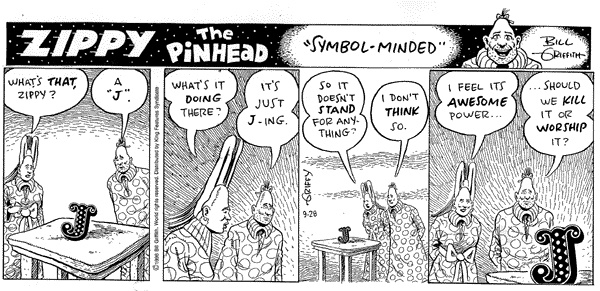
\includegraphics[width=0.8\textwidth]{zippy}
  \caption[Zippy the Pinhead]{Zippy\index{Zippy} \cite{zippy} isn't the only one challenged by the \emph{awesome power} of J.}
  \label{eps:zippy}
\end{figure}

\subsection{Whither Hungarian}

J is a \emph{dynamically typed} language!  What this means is that
you do not have to declare the types of arguments and that types
can change during program execution.  Discarding the 
type declaration machinery found in other programming languages simplifies
J coding but it can impose its own problems. Without declarations
it's not always clear \emph{what is a valid argument}.  J does
not require that you provide hints and, in J's \emph{tacit} case, it
does not even require that you provide arguments!  Given
the language's terse nature this quickly leads to an incomprehensible
style that J detractors have dubbed \emph{line noise}. 

To distinguish my J code from line noise I have adapted a documentation
style known as \href{https://en.wikipedia.org/wiki/Hungarian_notation}{Hungarian notation} \cite{wiki:hung}. 
 Hungarian notation inspires devotion and disgust.  Many swear by it and many
 swear at it.  For me a
convention is worthwhile if it \emph{helps me} understand code.  The style
outlined here helps me understand and maintain J code.  It might help you too.

\subsection{J Noun Types}

There are two broad classes of arguments in J: nouns and verbs.  Nouns are data;
they correspond to arguments found in other programming languages.  Verbs are programs.  J adverbs
and conjunctions take verb arguments.\footnote{Adverbs and conjunctions also take noun
arguments.} Adverbs and conjunctions roughly correspond to the
higher order functions found in languages like
\href{https://www.cs.cmu.edu/Groups/AI/html/cltl/cltl2.html}{\texttt{LISP}} \cite{commonlisp} and
\href{https://www-swiss.ai.mit.edu/projects/scheme/}{\texttt{Scheme}} \cite{scheme}. 
J \emph{explicit} definition syntax reserves the characters \texttt{x y m n
u v} for arguments: see Table~\ref{tab:jargs} on page~\pageref{tab:jargs}.\footnote{
Earlier versions of J used  \texttt{ x.\ y.\ m.\ n.\ u.\ v.\ } for arguments.  This inflected
syntax has been deprecated.} The Hungarian notation described here focuses on noun arguments, 
(\texttt{x} and \texttt{y}), because they are the most common.

\begin{table}[htbp]
  \centering
   \scriptsize
\begin{tabular}{|l|l|} \hline
   \multicolumn{2}{|c|}{\textbf{\normalsize J Explicit Arguments\T\B}} \\ \hline
   \texttt{x\T\B} & \textcolor{CodeComment}{\ttfamily\textsl{left verb noun argument}}  \\
   \texttt{y\T\B} & \textcolor{CodeComment}{\ttfamily\textsl{right verb noun argument}} \\ 
   \texttt{m\T\B} & \textcolor{CodeComment}{\ttfamily\textsl{left conjunction noun argument}} \\ 
   \texttt{n\T\B} & \textcolor{CodeComment}{\ttfamily\textsl{right conjunction noun argument}} \\ 
   \texttt{u\T\B} & \textcolor{CodeComment}{\ttfamily\textsl{left adverb/conjunction verb argument}} \\ 
   \texttt{v\T\B} & \textcolor{CodeComment}{\ttfamily\textsl{right conjunction verb argument}}  \\ \hline
\end{tabular}
   \caption[J Arguments]{Characters reserved for J \emph{explicit} definition arguments. \emph{Tacit} definitions do
   not directly refer to arguments.}
   \label{tab:jargs}
\end{table}

To succinctly describe a J noun you need to be mindful of:
\begin{itemize}
	\item Type
	\item Rank
	\item Boxing
\end{itemize}

\textbf{J types} are congruent to simple types in other languages.  The standard J utility verb \texttt{datatype} enumerates primitive J noun types.

\begin{lstlisting}[frame=single,framerule=0pt,basicstyle=\ttfamily\footnotesize] 
datatype=: 3 : 0
  n=. 1 2 4 8 16 32 64 128 1024 2048 4096 8192 16384 32768 65536 131072 262144
  n=. n,5 6 7 9 10 11
  t=. '/boolean/literal/integer/floating/complex/boxed/extended/rational'
  t=. t,'/sparse boolean/sparse literal/sparse integer/sparse floating'
  t=. t,'/sparse complex/sparse boxed/symbol/unicode/unicode4'
  t=. t,'/integer1/integer2/integer4/floating2/floating4/floating16'
  (n i. 3!:0 y) pick <;._1 t
)

  NB. types of list items
  datatype&.> (2x^128);1;'char';(s: ' symbol minded');7 %~ i. 4 5
+--------+-------+-------+------+--------+
|extended|boolean|literal|symbol|floating|
+--------+-------+-------+------+--------+
\end{lstlisting}  

\textbf{Rank} has a precise technical meaning in J but in this context it can be loosely
thought of as array dimension.   Typical ranks in J are:
\begin{itemize}
	\item Single numbers like \texttt{42} and characters \texttt{'a'} are called atoms. They
	have \textsl{rank 0}.\footnote{\textsl{Rank 0}, or \textsl{0-dimensional} objects occur in
	in all programming languages but are \emph{rarely recognized.} This leads to mountains of ugly special case code. J is more than a programming language; it's a comprehensive and rigorous way 
to \emph{think} about arrays.} 
	\item Lists like \verb|1 2 3| and \verb|'characters'| correspond to \textsl{1-dimensional} arrays
	in most languages and have \textsl{rank 1}.
	\item Tables like \verb|i. 3 2| are \textsl{2-dimensional} arrays and have \textsl{rank 2}.  
	\item $n$ dimensional arrays have rank $n$.
\end{itemize}

\textbf{Boxing} is structural.  J nouns are either boxed or simple.  A  simple noun
has one of the types, (excluding boxed), listed by
the \texttt{datatype} verb.  To mix types in a J array you must box.
\begin{lstlisting}[frame=single,framerule=0pt] 
      NB. you must box < to mix types in J arrays
      (<u: 'unicode me'),(<i. 2 3),<'types to mix'
\end{lstlisting}  

\subsection{Hungarian Noun Descriptions}

To describe J nouns I use the following rules:\footnote{As in
the film \emph{Pirates of the Caribbean} these rules are more like \emph{guidelines!}} 

\begin{figure}
  \centering
  \ttfamily
  \scriptsize
  \subfigure[J native type prefixes]{
\begin{tabular}{|l|l|l|} \hline
   \multicolumn{3}{|c|}{\rmfamily\textbf{\normalsize J Native Type Prefixes\T\B}} \\ \hline
   \multicolumn{1}{|c|}{\rmfamily\textbf{Prefix\T\B}} &
   \multicolumn{1}{|c|}{\rmfamily\textbf{Native Type\T\B}} &
   \multicolumn{1}{|c|}{\rmfamily\textbf{ \texttt{(3!:0)} code\T\B}} \\ \hline
 p\T\B & \textcolor{CodeComment}{\textsl{boolean}}   &      1  \\    
 c\T\B & \textcolor{CodeComment}{\textsl{literal}}   &      2  \\    
 i\T\B & \textcolor{CodeComment}{\textsl{integer}}   &      4  \\    
 f\T\B & \textcolor{CodeComment}{\textsl{floating}}  &      8  \\    
 j\T\B & \textcolor{CodeComment}{\textsl{complex}}   &      16 \\    
 b\T\B & \textcolor{CodeComment}{\textsl{boxed}}    &      32 \\    
 X\T\B & \textcolor{CodeComment}{\textsl{extended}}  &      64 \\    
 R\T\B & \textcolor{CodeComment}{\textsl{rational}}  &      128  \\  
 SP\T\B & \textcolor{CodeComment}{\textsl{sparse boolean}} & 1024  \\ 
 SC\T\B & \textcolor{CodeComment}{\textsl{sparse literal}} &  2048 \\  
 SI\T\B & \textcolor{CodeComment}{\textsl{sparse integer}} &  4096  \\ 
 SF\T\B & \textcolor{CodeComment}{\textsl{sparse floating}} & 8192 \\  
 SJ\T\B & \textcolor{CodeComment}{\textsl{sparse complex}}  & 16384 \\ 
 SB\T\B & \textcolor{CodeComment}{\textsl{sparse boxed}}    & 32768 \\ 
 s\T\B  & \textcolor{CodeComment}{\textsl{symbol}}          & 65536  \\                 
 w\T\B  & \textcolor{CodeComment}{\textsl{unicode}}         & 131072 \\ 
 W\T\B  & \textcolor{CodeComment}{\textsl{unicode4}}        & 262144 \\ \hline
\end{tabular}
  }
  \hspace{0.6cm} %\hfill
  \subfigure[Generic prefixes]{
  \begin{tabular}{|l|l|} \hline
   \multicolumn{2}{|c|}{\rmfamily\textbf{\normalsize Generic Prefixes\T\B}} \\ \hline
   \multicolumn{1}{|c|}{\rmfamily\textbf{Prefix\T\B}} &
   \multicolumn{1}{|c|}{\rmfamily\textbf{Description \T\B}} \\ \hline
 n\T\B & \textcolor{CodeComment}{\textsl{any numeric type including boolean}}  \\   
 N\T\B & \textcolor{CodeComment}{\textsl{any extended numeric type}}  \\
 u\T\B & \textcolor{CodeComment}{\textsl{universal - any J type}}  \\    
 z\T\B & \textcolor{CodeComment}{\textsl{empty - has at least one 0 axis}}  \\ \hline 
\end{tabular}
  }
  \caption[Hungarian Type Prefixes]{\rmfamily Hungarian type prefixes.}
  \label{fig:hungtype}
\end{figure}

\begin{enumerate}
	\item For basic descriptions I use \textsl{TypeRank[Name]}  where \textsl{Type} comes
	from Figure~\ref{fig:hungtype} on page~\pageref{fig:hungtype}, \textsl{Rank} is one of: 
	\begin{center}
	 \footnotesize
\begin{tabular}{ll}
   \texttt{a} & \textcolor{CodeComment}{\ttfamily\textsl{atom - rank 0}} \\ 
   \texttt{l} & \textcolor{CodeComment}{\ttfamily\textsl{list - rank 1}}  \\
   \texttt{t} & \textcolor{CodeComment}{\ttfamily\textsl{table - rank 2}} \\   
   \texttt{[n]} & \textcolor{CodeComment}{\ttfamily\textsl{general rank $n$}} \\ 
\end{tabular}
\end{center}
and \textsl{Name} is an optional descriptive name.  The \textsl{TypeRank} prefix uses
the case of Figure~\ref{fig:hungtype} on page~\pageref{fig:hungtype} and \textsl{Name} begins with an uppercase letter.
 \begin{center}
 \footnotesize
\begin{tabular}{ll}
   \texttt{paSwitch} & \textcolor{CodeComment}{\ttfamily\textsl{boolean (proposition) Switch}} \\ 
   \texttt{ilColors} & \textcolor{CodeComment}{\ttfamily\textsl{integer list Colors}}  \\
   \texttt{ctDocument} & \textcolor{CodeComment}{\ttfamily\textsl{character table Document}} \\   
   \texttt{jt} & \textcolor{CodeComment}{\ttfamily\textsl{complex numerix table or matrix}} \\ 
   \texttt{s[3]Xref} & \textcolor{CodeComment}{\ttfamily\textsl{rank 3 array of Xref symbols}} \\ 
   \texttt{Rl} & \textcolor{CodeComment}{\ttfamily\textsl{extended rational list}} \\ 
   \texttt{bt} & \textcolor{CodeComment}{\ttfamily\textsl{boxed table}} \\
   \texttt{SClRare} & \textcolor{CodeComment}{\ttfamily\textsl{sparse character list Rare}} \\
   \texttt{wlPersian} & \textcolor{CodeComment}{\ttfamily\textsl{unicode list Persian}} \\ 
   \texttt{ztHolder} & \textcolor{CodeComment}{\ttfamily\textsl{empty table Holder}} \\ 
   \texttt{ulWhatever} & \textcolor{CodeComment}{\ttfamily\textsl{universal list - any J list}} \\ 
   \texttt{uu} & \textcolor{CodeComment}{\ttfamily\textsl{universal universal - any J argument}} \\ 
\end{tabular}
\end{center}
 \item For boxed nouns of depth one I use a \textsl{TypeRankTypeRank[Name]} where the right most      pairing describes the boxed types.  Boxed nouns of depth one occur often.
 \begin{center}
 \footnotesize
\begin{tabular}{ll}
   \texttt{blcl} & \textcolor{CodeComment}{\ttfamily\textsl{boxed list of character lists}} \\ 
   \texttt{blit} & \textcolor{CodeComment}{\ttfamily\textsl{boxed list of integer tables}}  \\
   \texttt{bljtCoord} & \textcolor{CodeComment}{\ttfamily\textsl{boxed list of complex tables}} \\   
   \texttt{blul} & \textcolor{CodeComment}{\ttfamily\textsl{boxed list any lists}} \\ 
   \texttt{b[3]s[4]Maps} & \textcolor{CodeComment}{\ttfamily\textsl{boxed rank 3 array of rank 4 symbol array Maps }} \\ 
\end{tabular}
\end{center} 
 \item For more complex nouns, when it's helpful to expose some external structure, I use
 a mixture of more basic noun descriptions and J syntax. 
  \begin{center}
 \footnotesize
\begin{tabular}{ll}
   \texttt{(<blcl),<jtPlane} & \textcolor{CodeComment}{\ttfamily\textsl{two item list}} \\ 
   \texttt{pa;ftXy;<btuu} & \textcolor{CodeComment}{\ttfamily\textsl{three item list}}  \\
   \texttt{cl;ia;(<blcl),<blcl} & 
     \textcolor{CodeComment}{\ttfamily\textsl{see Table~\ref{tab:juses} page~\pageref{tab:juses}}} \\
   \texttt{itYYYYMMDD;slWords;(<bt),<clName} &
     \textcolor{CodeComment}{\ttfamily\textsl{four item list}} \\
   \texttt{saRed,saGreen,saBlue} & 
     \textcolor{CodeComment}{\ttfamily\textsl{emphasize items of simple noun}} \\
\end{tabular} 
\end{center}
 \item Finally, when more than one description is needed I separate individual 
 descriptions with the \emph{or} symbol \argsep and use as many consecutive lines as required.\footnote{The \argsep symbol was chosen because it falls outside 
 of J's ASCII vocabulary and suggests ``either-or.''} 
  \begin{center}
 \footnotesize
\begin{tabular}{l}
 \textcolor{CodeComment}{\ttfamily\textsl{dyadic \hyperlink{il:put}{put} argument description see page~\pageref{ss:put}}} \\
 \texttt{iaObject put clName \argsep blclNames \argsep btNvalues} \\
 \texttt{clLocale put clName \argsep blclNames \argsep btNvalues} \\
 \texttt{(iaObject,iaQualifier) put clName \argsep blclNames}  \\
 \texttt{(iaObject,iaQualifier) put clName \argsep btNvalues} \\
 \\
  \textcolor{CodeComment}{\ttfamily\textsl{dyadic \hyperlink{il:dnl}{dnl} argument description see page~\pageref{ss:dnl}}} \\
 \texttt{iaObject dnl zl \argsep clPstr} \\
 \texttt{(iaObject,iaOption) dnl zl \argsep clPstr} \\
  \texttt{(iaObject,iaOption,iaQualifier) dnl zl } \\
  \texttt{(iaObject,iaOption,iaQualifier) dnl clPstr} \\
\end{tabular} 
\end{center}
\end{enumerate}

\newpage
\section{JOD Mnemonics}

%\centering
\large
\itshape
  
\href{https://www.acronymfinder.com/Mnemonics-Neatly-Eliminate-Man's-Only-Nemesis-_-Insufficient-Cerebral-Storage-(MNEMONICS).html}{``\textbf{M}nemonics \textbf{N}eatly \textbf{E}liminate \textbf{M}an's \textbf{O}nly \textbf{N}emesis - \textbf{I}nsufficient \textbf{C}erebral \textbf{S}torage.''}

\Large

\begin{center}

	\hyperlink{il:jodhelp}{jodhelp} us!
	
	I \hyperlink{il:get}{get} it!

   \hyperlink{il:dnl}{dnl} is not just a river in Egypt.
   
   And Jesse \hyperlink{il:bget}{bget} old code.
	
	\hyperlink{il:put}{put} it where the sun don't shine.
	
	\hyperlink{il:make}{make} my day.

   \hyperlink{il:globs}{globs} of gunk.
	
	We're living in a golden \hyperlink{il:jodage}{jodage}.
	
	\hyperlink{il:did}{did}dle me this!
	
	\hyperlink{il:grp}{grp}'ing in the dark.
	
	Am I going to live \hyperlink{il:doc}{doc}?
	
	It was \hyperlink{il:revo}{revo}lting.
	
	He \hyperlink{il:od}{od}'ed man.
	
	\hyperlink{il:et}{et} phone home.
	
	It's a brand \hyperlink{il:newd}{newd}.
	
	He put on a fine \hyperlink{il:disp}{disp}lay.
	
	Dick \hyperlink{il:uses}{uses} Jane.
	
	I feel well \hyperlink{il:restd}{restd}.
	
	All \hyperlink{il:packd}{packd} up and nowhere to go.
	
	\hyperlink{il:bget}{bget} me a backup \href{https://www.youtube.com/watch?v=69iB-xy0u4A}{shrubbery}.
\end{center}

\normalsize	
\normalfont	

%\newpage
%\section{Web \texttt{URLS}}
%% urls embedded in document source.  This contents of this file
% has been derived from the output of J word (extracthrefs}
     
\begin{description}
                
\item  \emph{The JOD Pages}.\index{URL}  This website maintains references to all
JOD related documents and downloads.

\jodurl{http://bakerjd99.googlepages.com/home}
                                 
\item Wikipedia entry for \emph{Hungarian Notation}:  it's tedious and overwrought
but conveys the essentials.

\jodurl{http://en.wikipedia.org/wiki/Hungarian_notation}
                       
\item The website of the legendary computer scientist Donald Knuth.  Knuth created
the typesetting language \TeX\ in the
1970's and \TeX\ is still in widespread use because nothing
developed since is any better.  Genius is hard to replace!

\jodurl{http://www-cs-faculty.stanford.edu/~knuth/}
                            
\item All about the \emph{Scheme} programming language. 

 \jodurl{http://www-swiss.ai.mit.edu/projects/scheme/}
                          
\item \emph{Common Lisp} is the industrial strength version of the \texttt{LISP}
family of programming languages.  It's star has been waning since
the late 1980's.  

\jodurl{http://www.cs.cmu.edu/Groups/AI/html/cltl/cltl2.html}
                  
\item The  website for \emph{Graphviz}.  Graphviz is an amazing open source
system that draws graphs.  Some of the diagrams in this document were
generated with Graphviz using the J Graphviz addon.

\jodurl{http://www.graphviz.org}
                                               
\item J documentation for the \texttt{scriptdoc} utility.  

\jodurl{http://www.jsoftware.com/help/user/scriptdoc.htm}
                      
\item J Wiki download page for the \texttt{jodsource} addon.\index{Addon}

\jodurl{http://www.jsoftware.com/jwiki/Addons/general/jodsource}
               
\item J Wiki download page for the \texttt{jod} addon.

\jodurl{http://www.jsoftware.com/jwiki/Addons/general/jod}

\item J Wiki download page for the \texttt{graphviz} addon. After JOD this is
my favorite J addon. Oleg Kobchenko has created a jewel for J users!

\jodurl{http://www.jsoftware.com/jwiki/Addons/graphics/graphviz}

\item Oleg's J Page.  Chock full of interesting examples of J programming.

\jodurl{http://olegykj.sourceforge.net/}
                     
\item J Wiki addon list.  This is a complete list of J addons.

\jodurl{http://www.jsoftware.com/jwiki/Addons}
                                 
\item J Wiki documentation about JAL: the J package manager.  JAL is
the main tool for downloading and installing J addons. 

\jodurl{http://www.jsoftware.com/jwiki/JAL/Package_Manager}
                                              
\item Main J page.  This is were you go to download the latest version of J.  

\jodurl{http://www.jsoftware.com}
                                              
\item A hard copy spiral bound book version of this document is available 
here.  The price of the book is at cost. 

\jodurl{http://www.lulu.com/content/3229961}

\end{description}


%  
\newpage
\section{JOD Source Code}\label{ap:jodsource}

\begin{lstlisting}[frame=single,framerule=0pt,basicstyle=\ttfamily\tiny]
NB. jod.ijs -- main JOD dictionary class
NB.
NB. All other dictionary classes are extensions of the dictionary class.
NB. They all use standard constants and verbs defined in this class.
NB.
NB. Creating a JOD object defines a (z) locale interface.
NB. Destroying a JOD object erases the (z) locale interface.
NB.
NB. Contains: dictionary utilities, constants, interface verbs
NB.
NB. Interface: (verbs made available by z locale)
NB.   del     delete words, tests, groups, macros, et cetera
NB.   did     dictionary identification
NB.   dnl     dictionary name lists from patterns
NB.   dpset   sets dictionary parameters
NB.   gdeps   list group and suite dependents
NB.   get     get words, tests, macros, et cetera from dictionary
NB.   globs   word and test global name references
NB.   grp     create and query groups and suites
NB.   make    generate J scripts and database dumps
NB.   newd    create new dictionary
NB.   od      opens and closes dictionaries
NB.   packd   pack dictionaries
NB.   put     put words, tests, macros, et cetera into dictionary
NB.   regd    register/unregister a dictionary
NB.   restd   restore last backup created by (packd)
NB.   uses    words used by words and tests
NB.
NB. Notes:
NB.   Error messages (JOD errors 000-049)

coclass 'ajod'
require 'jfiles regex task'

NB.*dependents x-- words defined in this section have related definitions

NB. line feed, carriage return, tab and line ends
LF=:10{a.
CR=:13{a.
TAB=:9{a.
CRLF=:CR,LF

NB. option codes - to add more add a new object code
NB. and modify the following definition of MACROTYPE
JSCRIPT=:21
LATEX=:22
HTML=:23
XML=:24
TEXT=:25
UTF8=:26

NB. macro text types, depends on: JSCRIPT,LATEX,HTML,XML,TEXT,UTF8
MACROTYPE=:JSCRIPT,LATEX,HTML,XML,TEXT,UTF8

NB. object codes
WORD=:0
TEST=:1
GROUP=:2
SUITE=:3
MACRO=:4

NB. object name class, depends on: WORD,TEST,GROUP,SUITE,MACRO
OBJECTNC=:WORD,TEST,GROUP,SUITE,MACRO

NB. bad object code, depends on: OBJECTNC
badobj=:[: -. [: *./ [: , ] e. OBJECTNC"_

NB. path delimiter character & path punctuation characters
PATHDEL=:'\'
PATHCHRS=:' :.-',PATHDEL

NB. default master profile user locations
NB. jodsystempath is left global here as this
NB. verb is redefined in jod.ijs
JMASTER=:jodsystempath 'jmaster'
JODPROF=:jodsystempath 'jodprofile.ijs'
JODUSER=:jodsystempath 'joduserconfig.ijs'

NB.*enddependents
NB.*end-header

NB. valid characters in file and path names
ALPHA=:'ABCDEFGHIJKLMNOPQRSTUVWXYZabcdefghijklmnopqrstuvwxyz0123456789'

NB. master file cn: dictionary number log - see long documentation
CNMFDLOG=:10

NB. master file cn: in use bit
CNMFMARK=:0

NB. master file cn: dictionary parameter defaults
CNMFPARMDEFS=:9

NB. master file cn: dictionary parameters - see long documentation
CNMFPARMS=:7

NB. master file cn: main dictionary table - see long documentation
CNMFTAB=:2

NB. master file cn: main dictionary table backup
CNMFTABBCK=:3

NB. default option code
DEFAULT=:7

NB. comment tag marking end of dependents section
DEPENDENTSEND=:'enddependents'

NB. comment tag marking start of dependents section
DEPENDENTSSTART=:'dependents'

NB. document option code
DOCUMENT=:9

NB. controls dependent block processing - (1) process (0) do not process
DODEPENDENTS=:1

NB. dictionary path table - see long documentation
DPATH=:i.0 4

NB. maximum dictionary path length
DPLIMIT=:16


ERR001=:'invalid option(s)'
ERR002=:'invalid name(s)'
ERR003=:'name(s) to long'
ERR004=:'invalid or missing locale'
ERR005=:'invalid or missing dictionary name(s)'
ERR006=:'cannot read master'
ERR007=:'cannot read master documentation'
ERR008=:'invalid names(s) - embedded locale references'
ERR009=:'no documentation text for ->'
ERR010=:'invalid name pattern'
ERR011=:'error(s) creating dictionary master file'
ERR012=:'master in use - wait or try (dpset)'
ERR013=:'cannot mark master'
ERR014=:'invalid name and text'
ERR015=:'invalid name, class and text'
ERR016=:'definition failure among ->'
ERR017=:'jfile replace error'
ERR018=:'dictionary in use - cannot unregister'
ERR019=:'invalid parameter or value'
ERR020=:'table name(s) are not unique'
ERR021=:'dll error generating GUID'
ERR022=:'JOD z interface clashes with current z locale names. JOD load aborted'
ERR023=:'white space preservation is off - turn on to put'
ERR024=:'dependent section unbalanced'
ERR025=:'only one balanced dependent section allowed'
ERR026=:'error in joduserconfig.ijs - last J error ->'

NB. explain option code
EXPLAIN=:8

NB. minimum free space in bytes required to create dictionary
FREESPACE=:1048576

NB. database file extension (it's changed in the past)
IJF=:'.ijf'

NB. J script file extension
IJS=:'.ijs'

NB. inverted data code: name classes and macro types
INCLASS=:12

NB. inverted data code: object creation time
INCREATE=:13

NB. inverted data code: last object put time
INPUT=:14

NB. inverted data code: object size in bytes
INSIZE=:15

NB. core jod z interface words
IzJODinterface=:<;._1 ' del did dnl dpset gdeps get globs grp make newd od packd put regd restd uses'

NB. standard dictionary file names - order matters
JDFILES=:<;._1 ' jwords jtests jgroups jsuites jmacros juses'

NB. standard dictionary subdirectory names - order matters
JDSDIRS=:<;._1 ' script suite document dump alien backup'

NB. default JOD user directory
JJODDIR=:'joddicts\'

NB. regular expression matching valid J names
JNAME=:'[[:alpha:]][[:alnum:]_]*'


JODVMD=:'0.6.0';278;'20 Aug 2008 10:50:26'

NB. base J version - prior versions not supported by JOD
JVERSION=:,6.0199999999999996

NB. default master file parameters
MASTERPARMS=:6 3$'PUTFACTOR';'(+integer) words stored in one loop pass';100;'GETFACTOR';'(+integer) words retrieved in one loop pass (<2048)';250;'COPYFACTOR';'(+integer) components copied in one loop pass';100;'DUMPFACTOR';'(+integer) objects dumped in one loop pass (<240)';50;'DOCUMENTWIDTH';'(+integer) width of justified document text';61;'WWWBROWSER';'(character) browser command line - used for jod help';' "C:\Program Files\Internet Explorer\IEXPLORE.EXE"'

NB. maximum length of short explanation text
MAXEXPLAIN=:80

NB. maximum length of dictionary names
MAXNAME=:60

NB. (name,[class],value) option code
NVTABLE=:10

NB. successful return
OK=:1;1


OK001=:'dictionary unregistered ->'
OK002=:' is a noun - no references'
OK003=:'defaults restored for ->'
OK004=:'master file reset'
OK005=:'path cleared ->'
OK006=:'parameter set ->'
OK007=:'put dictionary is now a read/only library ->'
OK008=:'put dictionary read/write status restored ->'
OK009=:'put dictionary references deleted ->'

NB. indexes of dictionary subdirectories in dictionary parameter list
PARMDIRS=:4 5 6 7 8 9

NB. parameter file - extension is required
PARMFILE=:'jodparms.ijs'

NB. search pattern option codes
PATOPS=:1 2 3 _1 _2 _3

NB. controls whether words are saved when whitespace is discarded
PUTBLACK=:0

NB. reference option code
REFERENCE=:11

NB. maximum number of words per locale
SYMBOLLIM=:2048

NB. uses union option code
UNION=:31

NB. retains string after first occurrence of (x)
afterstr=:] }.~ #@[ + 1&(i.~)@([ E. ])

NB. trims all leading and trailing blanks
alltrim=:] #~ [: -. [: (*./\. +. *./\) ' '&=

NB. test for jfile append errors
badappend=:0: > {.


badblia=:4 : 0

NB.*badblia v-- returns 0 if (y) is a boxed list of integer atoms
NB. or singleton codes from (x)

if. _1 -: dat=. , (; :: _1:) y do. 1
elseif. (#y) ~: #dat do. 1
elseif. badil dat do. 1
elseif.do. -. *./ dat e. x
end.
)

NB. 1 if (y) is not boxed
badbu=:[: 32&~: 3!:0

NB. 1 if (y) is not a character list or atom
badcl=:-.@(2&=@(3!:0)) +. 1: < [: # $

NB. 1 if (y) is not a list of non-extended integers
badil=:-.@((([: # $) e. 0 1"_) *. 3!:0 e. 1 4"_)

NB. bad jfile read operation
badjr=:[: +./ _1 _2&e.

NB. bad locale name
badlocn=:[ >: [: 18!:0 ::(_2:) [: < ]

NB. bad return code
badrc=:[: -. 1: -: [: > {.

NB. test for jfile replacement errors
badreps=:0: > <./

NB. 1 if any of shape, type or sign differ
badsts=:0:

NB. 1 if items are not unique 0 otherwise
badunique=:# ~: [: # ~.

NB. retains string before first occurrence of (x)
beforestr=:] {.~ 1&(i.~)@([ E. ])

NB. boxes open nouns
boxopen=:<^:(L. = 0:)


catrefs=:3 : 0

NB.*catrefs v-- split into nonlocale and locale names.
NB.
NB. monad:  catrefs blcl

if. (,a:)-:,y do. ''
else.
  r=. islocref&> y  NB. insure 2 item result
  s=. <(-.r) # y
  l=. <r # y
  s,l
end.
)

NB. call dll
cd=:15!:0


changestr=:4 : 0

NB.*changestr v-- replaces substrings - see long documentation.
NB.
NB. dyad:  clReps changestr cl
NB.
NB.   NB. first character delimits replacements
NB.   '/change/becomes/me/ehh' changestr 'blah blah ...'

pairs=. 2 {."(1) _2 [\ <;._1 x      NB. change table
cnt=._1 [ lim=. # pairs
while. lim > cnt=.>:cnt do.         NB. process each change pair
  't c'=. cnt { pairs               NB. /target/change
  if. +./b=. t E. y do.             NB. next if no target
    u=. I. b                        NB. target starts
    'l m'=. #&> cnt { pairs         NB. lengths
    p=. u + 0,+/\(<:# u)$ d=. m - l NB. change starts
    s=. * d                         NB. reduce < and > to =
    if. s = _1 do.
      b=. 1 #~ # b
      b=. ((l * # u)$ 1 0 #~ m,l-m) (,u +/ i. l)} b
      y=. b # y
      if. m = 0 do. continue. end.  NB. next for deletions
    elseif. s = 1 do.
      y=. y #~ >: d u} b            NB. first target char replicated
    end.
    y=.(c $~ m *# u) (,p +/i. m)} y  NB. insert replacements
  end.
end. y                              NB. altered string
)


checknames=:3 : 0

NB.*checknames v-- tests alleged  boxed lists of J names. Accepts
NB. all valid J  names. When (x-:1)  names  with embedded locale
NB. references  are  rejected  otherwise  embedded   locales  are
NB. accepted.
NB.
NB. monad:  checknames cl|blcl
NB.
NB.   checknames 'we';'check';'out'
NB.
NB. dyad:  pa checknames cl|blcl
NB.
NB.   0 checknames ;:'accept our_poor_ locale__NAMES'

1 checknames y
:
msg=. ERR002  NB. errmsg: invalid name(s)
if. 1<#$ y        do. jderr msg return. end.
y=. ,&.> boxopen y   NB. allow char lists
if. +./ badcl&> y do. jderr msg return. end.

if. x do.
  NB. restrict embedded locales
  msg2=. ERR008  NB. errmsg: invalid names(s) - embedded locale references
  if. '_' e. , _1&{.&> y  do. jderr msg2 return. end.
  if. +./ +./@:('__'&E.)&> y do. jderr msg2 return. end.
  if. _2 e. nc y     do. jderr msg return. end.
else.
  NB. permit embedded locales - test must eschew class tests
  NB. to avoid evaluation of indirect locale references
  if. (#jnfrblcl y)~:#y do. jderr msg return. end.
end.

if. MAXNAME < >./ #&> y do. jderr ERR003 return. end. NB. errmsg: name(s) to long
ok trimnl y  NB. return deblanked name list
)


checknttab=:3 : 0

NB.*checknttab v--  checks (name,text)  tables. A name text table
NB. is a two column boxed table. Column 0  contains valid  names.
NB. Column 1 contains character  lists representing various texts
NB. like J scripts, LaTeX or HTML code.
NB.
NB. monad:  checknttab btcl
NB.
NB.  checknttab (;:'n1 n2 n3') ,. 'blah blah..';'more ehh..';'stuff ...'

msg =. ERR014 NB. errmsg: invalid name and text
if. badbu y do. jderr msg
elseif. -. 1 2 e.~ #$ y do. jderr msg
elseif. 2 ~: {: $ y=. plt y do. jderr msg
elseif. +./badcl&> 1 {"1 y do. jderr msg
elseif. badrc uv=.checknames (<a:;0){y do. jderr msg
elseif. badunique uv=. }.uv do. jderr ERR020
elseif.do. ok <y=. uv (<a:;0)} y  NB. insures deblanked names
end.
)


checknttab2=:4 : 0

NB.*checknttab2 v-- checks (name,class,text) tables.  Similar  to
NB. (checknttab)  except the  additional column is a numeric name
NB. class or type code.
NB.
NB. dyad:  ilCodes checknttab2 btcl
NB.
NB.  (i.4) checknttab2 'name';3;'verb=: ...'

msg=. ERR015 NB. errmsg: invalid name, class and text
if. badbu y do. jderr msg
elseif. -. 1 2 e.~ #$ y do. jderr msg
elseif. 3 ~: {: $ y=. plt y do. jderr msg
elseif. +./badcl&> {:"1 y do. jderr msg
elseif. x badblia 1 {"1 y do. jderr msg
elseif. badrc uv=.checknames (<a:;0){y do. jderr msg
elseif. badunique uv=. }.uv do. jderr ERR020
elseif.do. ok <y=. uv (<a:;0)} y  NB. insures deblanked names
end.
)


createjod=:3 : 0

NB.*createjod  v-- dictionary  object  creation  verb. (y) is  a
NB. dictionary object locale reference.  This verb initializes  a
NB. (z) locale user interface for the JOD system. and creates all
NB. necessary subobjects.
NB.
NB. monad:  paRc =. createjod ba
NB.
NB.   JD=: conew 'ajod'
NB.   createjod__JD JD


NB. set default master, profile and user if they don't exist
if. -.wex <'JMASTER' do. JMASTER=:jodsystempath 'jmaster' end.
if. -.wex <'JODPROF' do. JODPROF=:jodsystempath 'jodprofile.ijs' end.
if. -.wex <'JODUSER' do. JODUSER=:jodsystempath 'joduserconfig.ijs' end.

NB. set J version number 
JVERSION_ajod_=: (jvn :: _9:) ''  

NB. test JOD interface for z clashes
zwords=.(IzJODinterface,IzJODutinterface_ajodutil_) ,&.> locsfx 'z'
if. 1 e. uv=.0 <: nc zwords do.
  sp=. ] [ 1!:2&2
  0 [ sp ERR022,LF,LF,'z clashes:',LF,ctl list >uv#zwords

  NB. erase aborted dictionary object and jod classes
  coerase y
  0 [ coerase uv #~ 'ajod'&-:@:(4&{.)&> uv=. 18!:1 ] 0
  return.
end.

NB. create master file if necessary
if. -. fex <JMASTER,IJF do.
  if. badrc mdat=. createmast JMASTER do. mdat return. end.
end.

NB. execute any user script - allows for redefintions of various
NB. class nouns before JOD objects are created - joduserconfig.ijs
NB. is not installed and must be created by users
if. fex <JODUSER do. 
  NB. attempt execution of script
  if. (_9 -: ((0!:0) :: _9:) <JODUSER){0 1 do. (jderr ERR026),<13!:12 '' return. end.
end.

NB. initialize master dictionary parameters - used when
NB. creating directory objects to insure that all master
NB. parameters are set in directory objects - this amends
NB. the "jod" class to exploit inheritance in all derived classes
if. badjr mdat=. jread JMASTER;CNMFPARMS do. jderr ERR006 return. end.
MASTERPARMS_ajod_=: > mdat

NB. extension objects and complete (z) interface (*)=. JODEXT IZJODALL
JODEXT=: 0$a:
IZJODALL=: IzJODinterface,<'JODobj' 

NB. create storage, scratch, maker and utility objects !(*)=. JOD ST SO MK UT
JOD=: y
ST=: conew 'ajodstore'
MK=: conew 'ajodmake'
UT=: conew 'ajodutil'
SO=: cocreate ''    NB. empty classless object
obs=. JOD;ST;MK;UT;<SO

NB. initialize objects - they need to know each other
createst__ST obs
createmk__MK obs
createut__UT obs

NB. create direct _n_ (z) locale interface - if the (z)
NB. trap word (jodsf) exists define an error trapping interface
".&.> y defzface IzJODinterface

NB. attempt to create J temp directory ignoring errors
NB. required for JOD edit utilities and not always present on J systems
makedir <jpath '~temp\'

NB. execute any master dictionary profile script
if. fex <JODPROF do. (_9 -: ((0!:0) :: _9:) <JODPROF){1 0 else. 1 end.
)


createmast=:3 : 0

NB.*createmast v-- creates the dictionary master file. The master
NB. file  holds  the  master dictionary  directory and dictionary
NB. parameters. The master file tracks the state of dictionaries.
NB. In  this  system  only  one   task  can   open  a  dictionary
NB. read/write. When  opening a  dictionary  the master  file  is
NB. checked to  determine  if  the  dictionary  has  been  opened
NB. read/write  by  another  task.  Dictionaries  can  be  opened
NB. read/only by any number of tasks.
NB.
NB. monad:  createmast clFile
NB.
NB.   createmast_ajod_  JMASTER_ajod_  NB. recreate master

fn=.  y
syp=. PATHDEL ,~ (justdrv , ':'"_ , justpath) fn

if. badappend jcreate fn do.
  jderr ERR011 NB. errmsg: error(s) creating dictionary master file
  return.
end.

fn=. jopen_jfiles_ fn
cn=. (<0;now '') jappend fn     NB. c0 use bit and last change
'jodversion jodbuildcnt'=. 2{.JODVMD
cn=. cn, (<jodversion;jodbuildcnt,didnum 0) jappend fn  NB. c1 version, build #, unique id
cn=. cn, (4 0$'') jappend fn    NB. c2 dictionary directory
cn=. cn, (4 0$'') jappend fn    NB. c3 directory backup
cn=. cn, (3#<'') jappend fn     NB. c4,c5,c6 RESERVED

NB. parse parameter settings --- sets (MASTERPARMS)
0!:0 <syp,PARMFILE
parms=. <dptable MASTERPARMS    NB. created by 0!:0 !(*)=. MASTERPARMS

cn=. cn, parms jappend fn       NB. c7 active dictionary parameters
cn=. cn, parms jappend fn       NB. c8 active parameter backup
cn=. cn, parms jappend fn       NB. c9 default parameters
cn=. cn, (i.0) jappend fn       NB. c10 dictionary log
jclose_jfiles_ fn
if. 0 > <./cn do.
  jderr ERR011
else.
  ok {: cn  NB. return last component
end.
)

NB. character table to newline delimited list
ctl=:}.@(,@(1&(,"1)@(-.@(*./\."1@(=&' '@])))) # ,@((10{a.)&(,"1)@]))

NB. enclose all character lists in blcl in " quotes
dblquote=:'"'&,@:(,&'"')&.>


decomm=:3 : 0
                                                                 
NB.*decomm v--  removes comments  from j words. The (x) argument
NB. specifies whether all blank lines are removed or retained.   
NB.                                                              
NB. monad:  decomm ctWord                                        
NB.                                                              
NB.   decomm jcr 'decomm'  NB. decomment self                    
NB.                                                              
NB. dyad:  pa decomm ctWord                                      
NB.                                                              
NB.   1 decomm jcr 'decomm'  NB. remove blanks (default)         
NB.   0 decomm jcr 'decomm'  NB. retain all blank lines          
                                                                 
1 decomm y                                                      
:
NB. mask of unquoted comment starts                              
c=. ($y)$'NB.' E. ,y                                           
c=. +./\"1 c > ~:/\"1 y e. ''''                                 
y=. ,y                                                         
                                                                 
NB. blank out comments                                           
y=. ' ' (I. ,c)} y                                     
y=. y $~ $c                                                    
                                                                 
NB. remove blank lines - default                                 
if. x do. y #~ y +./ . ~: ' ' end.                            
)


defzface=:4 : 0

NB.*defzface v-- define z interface from word list.
NB.
NB. dyad:  blcl =. clSuffix defzface blclWords

if. 3 = (4!:0) <'jodsf_z_' do. 
  iface=. (y ,&.> locsfx x) ,&.> <' :: jodsf'
else.
  iface=. y ,&.> locsfx x
end.
(y ,&.> <'_z_=:') ,&.> iface
)


del=:3 : 0

NB.*del v-- deletes objects in dictionary database  files. Result
NB. is  a return code and message. The deletion only modifies the
NB. object's directory. The  actual data  remains in the file  as
NB. "dead"  components  until a (packd)  operation reclaims  file
NB. space.
NB.
NB. monad:  del blclWords
NB.
NB.   del ;: 'we are toast'
NB.
NB. dyad:  iaObject del blclName
NB.
NB.   1 del 'toast these tests'

WORD del y
:
msg=. ERR001
if. badil x do. jderr msg return. end.

NB. do we have a put dictionary open?
if. badrc uv=. checkput__ST 0 do. uv return. end.
DL=. 1 { uv

select. x
case. WORD do.
  (WORD;INVWORDS__ST;<DL) delstuff__ST y
case. TEST do.
  (TEST;INVTESTS__ST;<DL) delstuff__ST y
case. GROUP do.
  (GROUP;INVGROUPS__ST;<DL) delstuff__ST y
case. SUITE do.
  (SUITE;INVSUITES__ST;<DL) delstuff__ST y
case. MACRO do.
  (MACRO;INVMACROS__ST;<DL) delstuff__ST y
case. REFERENCE do.
  if. badrc y=. checknames y do. y
  elseif. badrc msg=. DL delwordrefs__ST }. y do. msg
  elseif.do. (ok OK009),<DNAME__DL
  end.
case. do. jderr msg
end.
)


destroyjod=:3 : 0

NB.*destroyjod v--  dictionary  object  destroy  verb.  This  verb
NB. erases the JOD (z) locale user interface.
NB.
NB. monad:  destroyjd uuIgnore

NB. close any open dictionaries
3 od ''

NB. erase current direct _n_ z locale references
NB. (*)=. IZJODALL JODEXT
(4!:55) IZJODALL ,&.> locsfx 'z'

NB. destroy sub-objects !(*)=. ST MK UT SO
coerase ST,MK,UT,SO

NB. destroy any JOD class extension objects
coerase JODEXT

NB. return self reference
18!:5 ''
)


did=:3 : 0

NB.*did v-- dictionary identification and statistics
NB.
NB. monad:  did uuIgnore
NB. dyad:  uuIgnore did uuIgnore

if. badrc msg=. checkopen__ST 0 do. msg else. ok {."1 DPATH__ST end.
:
0 didstats__ST 0
)


didnum=:3 : 0

NB.*didnum  v-- generates  a  unique  extended  precision integer
NB. based on the Win32 API GUID. The GUID is designed  to produce
NB. a  unique  global identifier every  time  it's  called.  This
NB. algorithm converts the GUID to a single  J extended precision
NB. integer to maintain compatibility with  the original (didnum)
NB. algorithm.
NB.
NB. NOTE: This algorithm is slower,  (about  1.5 milliseconds per
NB. DIDNUM),  than  (didnumoriginal) but  it  produces  a  better
NB. unique  identfier  besides  in  JOD  this verb is  called  so
NB. infreqently,  (once when  JOD is  loaded and once  when a new
NB. dictionary is created), that speed is not crucial. Uniqueness
NB. is far more important.
NB.
NB. monad:  didnumguid uuIgnore

NB. call dll to get GUID
guid=. genguid <16#' '
if. 0 ~: >{. guid do. jderr ERR021
else.
  NB. guid as 128 bit mask
  guid=. , (a. i. >{: guid){ truth 8

  NB. convert mask to an integer computing
  NB. only required extended powers of 2
  pos=. I. guid
  +/(2x ^ pos) pos} guid
end.
)


dnl=:3 : 0

NB.*dnl v-- list objects in dictionary database files.
NB.
NB. monad:  dnl clStr|zlStr
NB.
NB.   dnl ''        NB. list all words on path
NB.   dnl 'pfx'     NB. list all words on path begining with 'pfx'
NB.
NB. dyad:  ilCodes dnl clStr|zlStr
NB.
NB.   4 2  dnl 'ex'  NB. macros with names containing 'ex'
NB.   0 _1 dnl 'ugh' NB. path order listing of words ending with 'ugh'

WORD dnl y
:
if. badcl y do. jderr ERR010 return. end. NB. errmsg: invalid name pattern

msg0=. ERR001 NB. errmsg: invalid option(s)
if. badil x do. jderr msg0 return. end.

NB. do we have a dictionary open?
if. badrc msg1=.checkopen__ST 0 do. msg1 return. end.

NB. format standard (dnl) (x) options and search
x=.  x , (<:#x)}. 1 , DEFAULT
if. ({. x) e. OBJECTNC do. x dnlsearch__ST y else. jderr msg0 end.
)


dpset=:3 : 0

NB.*dpset v-- set dictionary parameters.
NB.
NB. monad:  dpset zl | clCommand | (cllParm ; uuValue)
NB. dyad:  iaCode dpset (clParm ; uuValue)

NB. objects !(*)=. DL ST

NB. resets should always work - close any open dictionaries
if. y -: 'RESETME' do.
  3 od '' NB. HARDCODE 3 close code
  if. badrc msg=. markmast~0 do. msg else. ok OK004 [ remast 1 end.
elseif. y -: 'RESETALL' do.
  3 od '' NB. HARDCODE 3 close code
  if. badrc msg=. markmast~0 do. msg else. ok OK004 [ remast 0 end.
elseif.do.
  NB. other options require an open dictionary
  if. badrc msg=.checkopen__ST 0 do. msg return. end.
  DL=.  {:{.DPATH__ST

  if. isempty y do.
    NB. display settable parameters of put/first with current values
    ok <|:>{:>jread WF__DL;CNPARMS__ST

  elseif. -.badcl y do.
    NB. if we are resetting READWRITE status dictionary need only be open
    if. 'READWRITE'-:y do.

      NB. check attributes of READONLY dictionary to insure 
      NB. that it will allow read/write operations on all files
      dcfiles=. (WF__DL;TF__DL;GF__DL;SF__DL;MF__DL;UF__DL) ,&.> <IJF
      NB. err msg (JODstore errors): dictionary file attributes do not allow read/write
      if. 0 e. iswriteable__ST dcfiles do. (jderr ERR095__ST),<DNAME__DL return. end.

      if. badrc msg=.libstatus__DL 0 do. msg
      else.
        RW__DL=: -. LIBSTATUS__DL=: 0  NB. library off/read write
        ok OK008;DNAME__DL
      end.
      return.
    end.
    NB. other changes of dictionary parameters require a put dictionary
    if. badrc msg=. checkput__ST 0 do. msg return. end.
    select. y
    case. 'DEFAULTS' do.
      if. badjr dat=. jread JMASTER;CNMFPARMDEFS   do. jderr ERR088
      elseif. badjr dpt=. jread WF__DL;CNPARMS__ST do. jderr ERR088
      elseif. dpt=. <(}:>dpt),<|: 1 0 1#"1 dat=. >dat
              badreps dpt jreplace WF__DL;CNPARMS__ST  do. jderr ERR017
      elseif.do.
        NB. reset live object parameters
        (({."1 dat) ,&.> locsfx DL)=: {:"1 dat
        ok OK003;DNAME__DL
      end.
    case. 'CLEARPATH' do.
      RPATH__DL=. i.0
      if. badreps (i.0) jreplace UF__DL;CNRPATH__ST do.
        jderr ERR017
      else.
        ok OK005;DNAME__DL
      end.
    case. 'READONLY' do.
      if. badrc msg=.libstatus__DL 1 do. msg
      else.
        RW__DL=: -. LIBSTATUS__DL=: 1  NB. library on/read only
        ok OK007;DNAME__DL
      end.
    case.do. jderr ERR001
    end.

  elseif. -.badbu y do.
    msg=. ERR019  NB. errmsg: invalid name/parameter
    if. -. (1=#$ y) *. 2=#y do. jderr msg return. end.
    if. badjr dpt=. jread WF__DL;CNPARMS__ST do. jderr ERR088 return. end.
    usp=. >{:dpt=. >dpt
    if. ({:$usp) = pos=. ({.usp) i. {.y do. jderr msg return. end.
    if. (>pos{{:usp) badsts >{:y do. jderr msg return. end.
    NB. reset live object
    ('__DL' ,~ >pos{{.usp)=: >{:y
    dpt=. (}:dpt),<usp=. ({:y) (<1;pos)} usp
    if. badreps (<dpt) jreplace WF__DL;CNPARMS__ST do. jderr ERR017 else. ok OK006;y end.

  elseif.do. jderr ERR001
  end.
end.
)


dptable=:3 : 0

NB.*dptable  v--  parses MASTERPARMS.
NB. 
NB. (MASTERPARMS) is set by running the script (jodparms.ijs).
NB.
NB. monad:  dptable clParms
NB.
NB.   0!:0 <jpath '~addons\general\jodparms.ijs'
NB.   dptable__JODobj  MASTERPARMS

NB. parse MASTERPARMS table - remove J comments
y=. (<;._1)"1  ';' ,. decomm ];._2 y -. CR

NB. remove extra blanks
y=. (alltrim&.>(<a:;0 1){y) (<a:;0 1)} y

NB. handle parm types currently only (+integer) and (character)
NB. NIMP - there is no error checking for dictionary parameters
ptype=. > 1{"1 y
pint=. I. (,:'(+integer)') ({."1)@E. ptype

NB. character and other types left as is
NB. char=. I. (,:'(character)') ({."1)@E. ptype
y=. (".&.> (<pint;2){y) (<pint;2)} y
)

NB. 1 if empty dictionary name list 0 otherwise
empdnl=:(,<0$0) -: ]

NB. test boxed list of path\file names for existence (0 some bad, 1 all ok)
fex=:*./@:(1:@(1!:4) ::0:)

NB. 0's all but the first 1 in runs of 1's
firstone=:] > [: }: 0: , ]

NB. first of doubles
fod=:] #~ 1 0"_ $~ #

NB. first on path order list index - see long documentation
fopix=:1: i.~ [ +/@:e.&> [: < [: < ]


gdeps=:3 : 0

NB.*gdeps v-- group and suite dependents.
NB.
NB. Dependents are global J assignments between the dependents tags:
NB.
NB. verbatim:
NB.
NB.    NB.*dependents
NB.    NB.*enddependents
NB.
NB. monad:  gdeps clGroup
NB.
NB.   gdeps 'jod'
NB.
NB. dyad:   iaGScode gdeps clGroupSuite
NB.
NB.   3 gdeps 

GROUP gdeps y
:
if. badil x     do. jderr ERR001 NB. errmsg: invalid options 
elseif. badcl y do. jderr ERR002 NB. errmsg: invalid name(s)
elseif.  x=. {.x
         -. x e. GROUP,SUITE do. jderr ERR001
elseif.  badrc uv0=. (x,1) obtext__UT y do. uv0 
elseif.do.
  uv0=. ,>2{uv0
  NB. hides tags from searches
  beg=. 'NB.*',DEPENDENTSSTART
  fin=. 'NB.*',DEPENDENTSEND
  tcnt=. (+/beg E. uv0),+/fin E. uv0 
  select. tcnt
  case. 0 0 do. ok ''
  case. 0 1 do. jderr ERR024  NB.errmsg: dependent block unbalanced
  case. 1 0 do. jderr ERR024
  case. 1 1 do.
     uv0=. ];._1 LF,fin beforestr uv0 -. CR
     0 namecats__MK uv0 }.~ I. (,:beg) +./"1@E. uv0
  case.do.
    jderr ERR025 NB. errmsg: only one balanced dependent block allowed
  end.
end.
)

NB. generates a GUID with dll call
genguid=:'ole32.dll CoCreateGuid i *c'&cd


get=:3 : 0

NB.*get v-- retrieves objects from dictionary database files.
NB.
NB. monad:  get blcl
NB.
NB.   get ;: 'us poor little words'
NB.
NB. dyad:  ilCodes get bluu
NB.
NB.   2 7 put 'GroupName';'Group documentation text ....'

WORD get y
:
msg=. ERR001 [ loc =. <'base' NB. errmsg: invalid option(s)

if. badil x do.
  NB. errmsg: invalid or missing locale
  if. _2&badlocn x do. jderr ERR004 return. else. x=. WORD [ loc=. <x-.' ' end.
end.

NB. do we have a dictionary open?
if. badrc uv=. checkopen__ST 0 do. uv return. end.

NB. format standard x. options
x=. x , (-3-#x) {. DEFAULT , 0
if. -. 0 1 e.~ {: x do. jderr msg return. end.

select. {. x
case. WORD do.
  select. second x
    case. DEFAULT  do. loc defwords__ST y
    case. EXPLAIN  do. WORD getexplain__ST y
    case. DOCUMENT do. WORD getdocument__ST y
    case. NVTABLE  do. (WORD,0) getobjects__ST y
    case. INCLASS;INCREATE;INPUT;INSIZE do. (2{.x) invfetch__ST y
    case.do. jderr msg
  end.
case. TEST do.
  select. second x
    case. DEFAULT  do. (TEST,0) getobjects__ST y
    case. EXPLAIN  do. TEST getexplain__ST y
    case. DOCUMENT do. TEST getdocument__ST y
    case. INCREATE;INPUT;INSIZE do. (2{.x) invfetch__ST y
    case.do. jderr msg
  end.
case. GROUP do.
  select. second x
    case. DEFAULT  do. GROUP getgstext__ST y
    case. EXPLAIN  do. GROUP getexplain__ST y
    case. DOCUMENT do. GROUP getdocument__ST y
    case. INCREATE;INPUT do. (2{.x) invfetch__ST y
    case.do. jderr msg
  end.
case. SUITE do.
  select. second x
    case. DEFAULT  do. SUITE getgstext__ST y
    case. EXPLAIN  do. SUITE getexplain__ST y
    case. DOCUMENT do. SUITE getdocument__ST y
    case. INCREATE;INPUT do. (2{.x) invfetch__ST y
    case.do. jderr msg
  end.
case. MACRO do.
  select. second x
    case. DEFAULT  do. (MACRO,0) getobjects__ST y
    case. EXPLAIN  do. MACRO getexplain__ST y
    case. DOCUMENT do. MACRO getdocument__ST y
    case. INCLASS;INCREATE;INPUT;INSIZE do. (2{.x) invfetch__ST y
    case.do. jderr msg
  end.
case.do. jderr msg
end.
)


globals=:4 : 0
if. badcl y do. jderr ERR002 return. end. NB. errmsg: invalid name(s)
if. badrc y=. 0 checknames y do. y
else.
  y =.>1{y
  NB. use base locale if no locale reference
  if. -.islocref y do. y=. y,'_base_' end.
  x wrdglobals__MK y
end.
)


globs=:3 : 0

NB.*globs v-- analyze, report and store global names
NB.
NB. monad:  globs clName
NB.
NB.   globs 'word'    NB. list globals in locale word
NB.
NB. dyad:   iaCode globs clName
NB.
NB.   NB. stores global references of word in dictionary
NB.   0 globs 'word'
NB.
NB.   1 globs 'test'  NB. list globals in test

0 globals y
:
if. (,x)-:,REFERENCE do. 1 globals y
elseif. badcl y do. jderr ERR002 NB. errmsg: invalid name(s)
elseif.do.
  select. x
  case. WORD do.
    if. badrc uv=. checkput__ST 0  do. uv return. else. DL=. 1 { uv end.
    if. badrc y=. checknames__ST y do. y return. else. y=. ,>}.y end.
    if. badrc uv=. (WORD;<DL) inputdict__ST <y  do. uv return. end.
    if. badrc uv=. WORD getobjects__ST y do. uv return. else. uv=. ,1 {:: uv end.
    if. 0=>1{uv do. ok '<',y,'>',OK002 return. end.
    if. badrc uv=. 0 namecats__MK ];._2 (>2{uv),LF do. uv return. end.
    (y;<DL) putwordxrs__ST }.uv
  case. TEST do.
    if. badrc uv=. TEST get y do. uv return. else. uv=. ,1 {:: uv end.
    NB. return references in stored test text
    0 namecats__MK ];._2 (>1{uv),LF
  case.do. jderr ERR001  NB. errmsg: invalid option(s)
  end.
end.
)


grp=:3 : 0

NB.*grp v-- create and modify groups.
NB.
NB. monad:  grp blcl
NB. dyad: ia grp ?

GROUP grp y
:
select. x
  case. GROUP do. (GROUP,WORD) gsmakeq y
  case. SUITE do. (SUITE,TEST) gsmakeq y
  case.do. jderr ERR001 NB. errmsg: invalid option(s)
end.
)


gsmakeq=:4 : 0

NB.*gsmakeq v-- make or query groups and suites.
NB.
NB. dyad:  ilCodes gsmakeq blcl

'gscode obcode'=. x

if. isempty y do. gscode dnl ''
else.
  if. badcl y do.

    NB. create/modify group
    if. badrc mdl=. checkput__ST 0  do. mdl return. end.
    if. badrc msg=. checkpath__ST {: mdl do. msg return. end.
    NB. remove empties from name list allows (grp 'name';'') to create null groups
    if. badrc y=.  checknames y -. a: do. y return. end.
    (({:mdl);obcode;gscode) putgs__ST }. y

  else.

    NB. query group contents
    if. badrc msg=. checkopen__ST 0 do. msg return. end.
    if. badrc y=. checknames y do. y return. end.
    gscode gslistnl__ST rv y
  end.
end.
)

NB. 1 if noun is empty on any axis and 0 otherwise
isempty=:0: e. $

NB. 1 if name is a locale reference 0 otherwise
islocref=:('_'"_ = {:) +. [: +./ '__'"_ E. ]

NB. error trapped call to jappend_jfiles_
jappend=:jappend_jfiles_ ::(_2:)

NB. character table representation of j words, call:  jcr 'verb'
jcr=:[: ];._1 (10{a.) , [: 5!:5 <

NB. error trapped call to jcreate_jfiles_
jcreate=:jcreate_jfiles_ ::0:

NB. format error message
jderr=:0: ; '!JOD error: '"_ , ]


jdmasterr=:3 : 0

NB.*jdmasterr v-- master error handling.
NB.
NB. Use when the master file is set otherwise the master will not
NB. be  properly reset. Because of the file overhead I decided to
NB. use a second error  handler  instead  of  burdening the  very
NB. frequently called  (jderr)  with this  often unnecessary file
NB. access function.

if. badrc msg=.markmast~0 do. msg else. jderr y end.
)


jnfrblcl=:3 : 0

NB.*jnfrblcl  v-- extracts valid  J names  from  boxed  lists  of
NB. character lists. Only  proper  unquoted,  inflection free (no
NB. trailing .'s)  names are  returned. This  verb extracts names
NB. without using name class tests. Class tests cannot be used on
NB. indirect locale names, eg. (BOO__HOO)  as the noun (HOO) must
NB. exist.
NB.
NB. monad: jnfrblcl  blcl
NB.
NB.   jnfrblcl 'good';' '' bad';'888';'ok';'notok.';'3r7'

NB. trim end blanks and eliminate any empties
y=. y #~ 0 < #&> y=.alltrim&.> y

NB. remove all lists containing invalid name characters
y=. y #~ y *./@:e.&> <ALPHA,'_'

NB. remove all lists beginning with numerals and _
y=. y #~ -.({.&> y) e. '_0123456789'

NB. extract any remaing names with regular expression
NB. NOTE: The way regular expressions are implemented differs
NB. in J4.05 from previous J systems.  The verb rxall is part
NB. of the regular expression system.  It is referred to without
NB. locale qualifications to support new and old J systems.
if. #y do. JNAME rxall ; y ,&.> ' ' else. '' end.
)

NB. error trapped call to jread_jfiles_
jread=:jread_jfiles_ ::(_2:)

NB. error trapped call to jreplace_jfiles_
jreplace=:jreplace_jfiles_ ::(_2:)

NB. extracts the drive from qualified file names
justdrv=:[: }: ] #~ [: +./\. ':'&=

NB. extracts only the path from qualified file names
justpath=:[: }: ] #~ ([: -. [: +./\. ':'&=) *. [: +./\. '\'&=


jvn=:3 : 0

NB.*jvn-- J version number.
NB.
NB. monad:  na =. jvn uuIgnore

NB. J version number
ver=. 9!:14 ''
ver=. (ver e. '0123456789/')#ver

NB. return version 6.01 if string is not numeric
100 %~ , 601 ". (ver i. '/') {. ver
)

NB. removes all leading and trailing CR and LF characters
lfcrtrim=:] #~ [: -. [: (*./\. +. *./\) ] e. (10 13{a.)"_

NB. surround names with locale delimiters, eg: _name_
locsfx=:'_'&,@,&'_'&.>


make=:3 : 0

NB.*make v-- makes J scripts.
NB.
NB. monad:  make zl|cl
NB.
NB.   make ''  NB. basic put dump
NB.
NB. dyad:  ilObjOpt make cl|blcl
NB.
NB.   0 make ;:'an arbitrary list of words into a script and file it'
NB.   0 2 make ;: 'a list of words returned as a character list'
NB.
NB.   3 make 'suite'    NB. make suite write to script subdirectory
NB.   2 2 make 'group'  NB. make group return character list
NB.
NB.   NB. make groups that are not in put dictionary
NB.   NB. file is written to put dictionary script directory
NB.   2 _1 make 'deepgroup'

makedump__MK y
:
msg=. ERR001  NB. errmsg: invalid option(s)
if. badil x do. jderr msg return. end.

NB. do we have a dictionary open?
if. badrc uv=. checkopen__ST 0 do. uv return. end.

NB. format standard (x) options HARDCODE
x=. 2 {. x , 1 2
if. -.({: x) e. _2 _1 1 2 do. jderr msg return. end.

if. ({. x) e. GROUP,SUITE do. x makegs__MK y
elseif.  ({. x)=WORD do.
  if. badrc uv=.WORD obtext__UT y do. uv
  elseif. 1={: x do. (WORD;1{uv) writeijs__MK >{:uv
  elseif.do. ok >{: uv
  end.
elseif.do. jderr msg
end.
)

NB. make a directory (1 success, 0 failure)
makedir=:1!:5 ::0:


markmast=:3 : 0

NB.*markmast v-- marks the master dictionary file. This system is
NB. is primarily  a single  writer  system. Many dictionary tasks
NB. can read data but only one  task can  change  it.  The master
NB. file  is used to enforce this  protocol. (markmast)  sets and
NB. unsets a use bit. When the bit is set the master file  itself
NB. cannot be changed.
NB.
NB. monad:  markmast uuIgnore
NB. dyad:   uuIgnore markmast uuIgnore

NB. set the use bit/timestamp in the master file
if. badjr ub=. jread JMASTER;CNMFMARK do. jderr ERR006  NB. errmsg: cannot read master
elseif. >{.>ub do. jderr ERR012  NB. errmsg: master in use - wait or try (dpset)
elseif. badreps (mubmark y) jreplace JMASTER;CNMFMARK do.
  jderr ERR013 NB. errmsg: cannot mark master
elseif.do. ok y
end.
:
NB. dyad resets the master
if. badreps (mubmark 0) jreplace JMASTER;CNMFMARK do. jderr ERR013 else. ok 0 end.
)

NB. master use bit mark
mubmark=:] ; [: (6!:0) 0: $ ]

NB. J name class
nc=:4!:0


newd=:3 : 0

NB.*newd v-- creates a new dictionary
NB.
NB. monad:  newd clName | (clName ; clPath)
NB.
NB.  newd 'New Dictionary'  NB. store in default J user directory
NB.  newd 'Newer Dictionary';'c:\put\it\here'  NB. drive required

if. badcl y do.
  1 newregdict__ST y
else.
  drn=. y -. y -. ALPHA  NB. safe directory chars only
  1 newregdict__ST y;(jpath '~user\'),JJODDIR,(255<.#drn){.drn
end.
)

NB. numeric list timestamp
now=:6!:0

NB. convert timestamp to yyyymmdd
nowfd=:([: 0 100 100&#. 3: {. ]) + ([: 24 60 60&#. 3: }. ]) % 86400"_


obidfile=:3 : 0

NB.*obidfile v-- location of jod object id history file.
NB.
NB. monad: obidfile uuIgnore

(jodsystempath ''),'jod.ijn'
)


od=:3 : 0

NB.*od v-- opens and closes dictionaries.
NB.
NB. monad: od clDictionary|blclDictionary
NB.
NB. dyad:  iaOption od clDictionary|blclDictionary
NB.
NB.   od 'test dictionary';'another test dictionary'  NB. open r/w
NB.   3 od 'test dictionary'                          NB. close

1 od y
:
msg=. ERR005 NB. errmsg: invalid or missing dictionary names

NB. list all registered dictionaries (short form)
if. badjr mdt=. jread JMASTER;CNMFTAB do.
  jderr ERR006 return.
end.
dl=. 0{>mdt

select. x
case. 1 do.   NB. HARDCODE: magic numbers read/write codes

  if. isempty y do. ok /:~ dl
  else.
    NB. open read/write
    y=. boxopen ,y
    NB. all dictionary names must be on master list
    if. *./y e. dl do. y opendict__ST 1;mdt else. jderr msg end.
  end.

case. 2 do.

  NB. open read/only
  y=. boxopen ,y
  if. *./y e. dl do. y opendict__ST 2;mdt else. jderr msg end.

case. 3 do.

  NB. close dictionaries
  if. badrc msg1=. checkopen__ST 0 do. msg1 return. end.
  if. isempty y do. y=. {."1 DPATH__ST else. y=.boxopen ,y end.
  if. *./y e. dl do. mdt closedict__ST y else. jderr msg end.

case. 4 do.

  NB. HARDCODE (mdt rows) display dictionary names and source paths
  mdt=. 0 2{>mdt
  ok <(/:0{mdt){ |: mdt

case. 5 do. 

  NB. return the currently registered dictionaries as a (regd) script
  mdt=. quote&.> 0 2{>mdt
  mdt=. ctl ;"1 (<'regd ') ,"1 |: 1 0 2{ (<';'),mdt
  NB. prefix command to close and unregister all current dictionaries
  mdt=. '3 regd&> }. od'''' [ 3 od ''''',LF,mdt
  ok 'NB. JOD registrations: ',(tstamp ''),LF,mdt
  

case.do. jderr ERR001  NB. errmsg: invalid option(s)
end.
)

NB. format normal return
ok=:1: ; ]


packd=:3 : 0

NB.*packd  v-- backs up and recovers wasted  space in  dictionary
NB. files.   Backups  are  stored  in  the   dictionary's  backup
NB. directory. Sets  of backup  files are prefixed  with an  ever
NB. increasing backup number, e.g: 13jwords.ijf. Dictionary files
NB. are NEVER deleted by JOD commands.
NB.
NB. monad:  packd clName
NB.
NB.   packd 'dictionary'

NB. only put dictionaries can be packed
if. badrc uv=. checkput__ST 0 do. uv return. end.
DL=. 1 { uv  NB. directory object !(*)=. DL

NB. is there enough space on the backup volume?
if. badrc uv=. packspace__DL 0 do. uv return. end.

packdict__DL y
)

NB. promote lists to tables - other ranks unchanged
plt=:]`,:@.(1&=@:(#@:$))


put=:3 : 0

NB.*put v-- stores objects in dictionary database files.
NB.
NB. monad:  put blclWords
NB.
NB.   put ;: 'it where the sun dont shine'
NB.
NB. dyad:  ilCodes put bluu
NB.
NB.   2 7 put 'GroupName';'Group documentation text ....'

WORD put y
:
msg=. ERR001 [ loc=. <'base'  NB. errmsg: invalid option(s)

NB. do not save decommented words - set PUTBLACK to 1 to override
if. -. PUTBLACK +. 9!:40'' do.
  NB. errmsg: white space preservation is off - turn on to put
  jderr ERR023 return.
end.

if. badil x do.
  NB. errmsg: invalid or missing locale
  if. _1&badlocn x do. jderr ERR004 return. else. x=. WORD [ loc =. <x-.' ' end.
end.

NB. do we have a put dictionary open?
if. badrc uv=. checkput__ST 0 do. uv return. end.
DL=. 1 { uv  NB. directory object !(*)=. DL

NB. format standard x. options
x=. 2 {. x , DEFAULT

select. {. x
case. WORD do.
  select. second x
    case. DEFAULT  do. (loc;<DL) putwords__ST y
    case. EXPLAIN  do. (WORD;<DL) putexplain__ST y
    case. DOCUMENT do. (WORD;1;<DL) puttexts__ST y
    case. NVTABLE  do.
      if. badrc y=. (i. 4) checknttab2 y do. y else. (WORD;<DL) puttable__ST y end.
    case.do. jderr msg
  end.
case. TEST do.
  select. second x
    case. DEFAULT  do.
      if. badrc y=. checknttab y do. y else. (TEST;<DL) puttable__ST y end.
    case. EXPLAIN  do. (TEST;<DL) putexplain__ST y
    case. DOCUMENT do. (TEST;1;<DL) puttexts__ST y
    case.do. jderr msg
  end.
case. GROUP do.
  select. second x
    case. DEFAULT  do. (GROUP;0;<DL) puttexts__ST y
    case. EXPLAIN  do. (GROUP;<DL) putexplain__ST y
    case. DOCUMENT do. (GROUP;1;<DL) puttexts__ST y
    NB. HARDCODE - lines inserted to maintain put/get symmetry for
    NB. the frequent argument cases 2 1 and 3 1 
    case. 1 do. (GROUP;0;<DL) puttexts__ST y
    case.do. jderr msg
  end.
case. SUITE do.
  select. second x
    case. DEFAULT  do. (SUITE;0;<DL) puttexts__ST y
    case. EXPLAIN  do. (SUITE;<DL) putexplain__ST y
    case. DOCUMENT do. (SUITE;1;<DL) puttexts__ST y
    case. 1 do. (SUITE;0;<DL) puttexts__ST y  NB. HARDCODE
    case.do. jderr msg
  end.
case. MACRO do.
  select. second x
    case. DEFAULT  do.
      if. badrc y=. MACROTYPE checknttab2 y do. y else. (MACRO;<DL) puttable__ST y end.
    case. EXPLAIN  do. (MACRO;<DL) putexplain__ST y
    case. DOCUMENT do. (MACRO;1;<DL) puttexts__ST y
    case.do. jderr msg
  end.
case.do. jderr msg
end.
)

NB. quotes character lists for execution
quote=:''''&,@(,&'''')@(#~ >:@(=&''''))

NB. reads a file as a list of bytes
read=:1!:1&(]`<@.(32&>@(3!:0)))

NB. reads a J binary noun file
readnoun=:3!:2@(1!:1&(]`<@.(32&>@(3!:0))))


readobid=:3 : 0

NB.*readobid  v--  unique  object ids  that  opened  dictionaries
NB. read/write on this machine.
NB.
NB. monad: readobid uuIngnore

(readnoun :: ((i.0)"_)) obidfile 0
)


regd=:3 : 0

NB.*regd v-- register and unregister JOD dictionaries.
NB.
NB. monad:  regd blcl
NB.
NB.   regd 'name';'c:\location\of\files';'documentation...'
NB.
NB. dyad:  iaOption make cl
NB.
NB.   3 regd 'name'  NB. unregister dictionary

0 newregdict__ST y
:
if. x-:3 do. NB. HARDCODE option
  NB. errmsg: invalid or missing dictionary name(s)
  if. badcl y do. jderr ERR005 return. end.
  NB. errmsg: dictionary in use - cannot unregister
  if. (<,y) e. {."1 DPATH__ST do. jderr ERR018 return. end.
  NB. errmsg: cannot read master
  if. badjr mdt=. jread JMASTER;CNMFTAB do. jderr ERR006 return. end.
  mdt=.>mdt
  mu=. (0{mdt)=<,y
  if. +./mu do.
    'path inuse'=. 2 3{mu #"1 mdt
    NB. errmsg: dictionary in use - cannot unregister
    if. inuse do. jderr ERR018 return. end.
    newmdt=. (-.mu)#"1 mdt
    if. badrc msg=. markmast 1 do. msg return. end.
    if. badreps ((<newmdt),<mdt) jreplace JMASTER;CNMFTAB,CNMFTABBCK do.
      jdmasterr ERR017 return.  NB. errmsg: jfile replace error
    end.
    if. badrc msg=. markmast~0 do. msg return. end.
    (ok OK001),y;,path
  else.
    jderr ERR005
  end.
else.
  jderr ERR001
end.
)


remast=:3 : 0

NB.*remast v-- clears all  in use bits  in the  master file. When
NB. JOD  opens a dictionary  an in  use bit is set in the  master
NB. file. When the dictionary  is closed the bit is cleared. When
NB. the  in  use  bit is set  the  dictionary  cannot  be  opened
NB. read/write by other dictionary tasks.
NB.
NB. monad:  remast paMeAll
NB.
NB.   remast 0  NB. reset all
NB.   remast 1  NB. reset me

mdt=. > jread JMASTER;CNMFTAB
if. 0=y do.
  NB. reset all
  mdt=. (<"0 ({:$mdt)#0) 3} mdt
else.
  NB. reset me
  mdt=. (<0) (<3;I. (;3{mdt) e. readobid obidfile 0)}mdt
end.
(<mdt) jreplace JMASTER;CNMFTAB
)


restd=:3 : 0

NB.*restd v-- restores the most recent backup created by (packd).
NB.
NB. monad:  restd cl
NB.
NB.   restd 'backup'

NB. only put dictionaries can be restored
if. badrc uv=. checkput__ST 0 do. uv return. end.
DL=. 1 { uv  NB. directory object !(*)=. DL

NB. is there enough space on the dictionary volume?
if. badrc uv=. restspace__DL 0 do. uv else. (}. uv) restdict__DL y end.
)

NB. ok return value
rv=:>@(1&{)


saveobid=:3 : 0

NB.*saveobid v--  saves the last  n JOD object ids  in the \jnxxx
NB. directory. These globally unique values are used to reset any
NB. dictionaries left open by JOD tasks spawned from  the current
NB. machine.
NB.
NB. monad:  saveobid xiObid
NB.
NB.   saveobid JODOBID

id=. ~. y , readobid file=.obidfile 0

NB. HARDCODE up to 30 last object ids spawned on this machine
NB. NOTE: if you run more than 30 JOD tasks on the current
NB. machine you will lose object id's which cause the RESETME
NB. option of (dpset) to not reset all dictionaries recently opened -
NB. but never closed - on this machine. JUST INCREASE THE NUMBER EHHH!!
((30<.#id) {. id) (writenoun :: _1:) file
)

NB. second list item
second=:1&{

NB. J type code
tc=:3!:0

NB. removes blanks from items on blcl
trimnl=:-.&' '&.>

NB. nth order truth table
truth=:#:@i.@(2&^)


tstamp=:3 : 0
NB.*tstamp v-- time stamp
yy=. <.y,(0=#y)#6!:0 ''
'yy m d h n s'=. 6{.yy
mth=. _3[\'   JanFebMarAprMayJunJulAugSepOctNovDec'
f=. _2: {. '0'&,@":
t=. (2":d),(m{mth),(":yy),;f&.>h,n,s
r=. 'xx xxx xxxx xx:xx:xx'
t (I. r='x') } r
)


uses=:3 : 0

NB.*uses v-- returns word references.
NB.
NB. monad:  uses blclName
NB.
NB.   NB. non-locale global word references
NB.   uses ;:'out global references please'
NB.
NB. dyad:   ilObjOpt uses clName
NB.
NB.   NB. global locale word references
NB.   11 uses ;:'out locale references'
NB.
NB.   0 31 uses 'wordname'  NB. uses union of word
NB.   0 32 uses '

0 uses y
:

if. badrc uv=. checkopen__ST 0 do. uv return. end.
if. badrc y=.checknames y do. y return. else. y=. }.y end.

msg=. ERR001 NB. errmsg: invalid option(s)
if. badil x do. jderr msg return. else. x=. ''$x end.

if. x-:WORD do.
  if. badrc dat=.WORD getrefs__ST y do. dat return. end.
  dat=. rv dat
  dat=. (uv=. {."1 dat) ,. > {:"1 dat
  NB. return in order requested
  ok <(({."1 dat) i. y){dat
elseif. x-:UNION do.

  NB. word uses unions
  uv=. i. 0 0
  for_wrd. y do.
    srch=.'' [ refs=.wrd
    loc=.'' [ self=.0
    while.do.
      if. badrc dat=.WORD getrefs__ST refs do. dat return. end.
      srch=. ~. srch , {."1 dat=. rv dat
      NB. only non-locale names are searched
      self=. self+.wrd e. new=. ~. ; {.&> {:"1 dat
      new=. new -. srch
      loc=. ~. loc , (; {:&> {:"1 dat) -. loc
      if. isempty new do. break. end.
      refs=. new
    end.
    srch=. /:~ srch -. self}.wrd
    uv=. uv,wrd,srch;<loc
  end.
  ok <uv

elseif.do. jderr msg
end.
)

NB. 1 when word with name exists 0 otherwise
wex=:0&<:@:nc

NB. word storage representation - nouns binary others linear
wrep=:5!:5@<`(3!:1@:".)@.(0&=@(nc@<))

NB. writes a list of bytes to file
write=:1!:2 ]`<@.(32&>@(3!:0))

NB. writes a J noun file
writenoun=:([: 3!:1 [) (1!:2 ]`<@.(32&>@(3!:0))) ]
\end{lstlisting}


	
